\documentclass[12pt]{article}

\usepackage{amsmath, amssymb, amsthm, amsfonts}
\usepackage{geometry}
\usepackage{microtype}
\usepackage{hyperref}
\usepackage{setspace}
\usepackage{titlesec}
\usepackage{mathtools}
\usepackage{tikz}
\usepackage{pgfplots}
\pgfplotsset{compat=1.18}
\usetikzlibrary{cd}

\geometry{margin=1.2in}
\onehalfspacing

\title{Thermodynamic Reachability\\
\large Geometric Bayesianism with Sparse Heuristics in Dynamically Constrained Systems}

\author{Flyxion}
\date{\today}

\theoremstyle{plain}
\newtheorem{theorem}{Theorem}[section]
\newtheorem{proposition}[theorem]{Proposition}
\newtheorem{lemma}[theorem]{Lemma}

\newtheorem{corollary}[theorem]{Corollary}

\theoremstyle{definition}
\newtheorem{definition}[theorem]{Definition}

\theoremstyle{remark}
\newtheorem{remark}[theorem]{Remark}

\begin{document}

\maketitle

\begin{abstract}
Standard models of inference assume that a system evaluates hypotheses drawn from a fixed and globally accessible space under an explicitly encoded prior. This work rejects that assumption and develops an alternative framework grounded in physical constraint. It is shown that thermodynamic limitations induce a time-dependent, reachability-limited hypothesis class, in which only functions constructible via energetically admissible, rate-bounded trajectories in state space are realizable. Apparent sparsity in representation emerges as a projection of this deeper constraint on trajectory complexity. This leads to a reformulation of Bayesian inference as constrained geometric flow on a dynamically evolving manifold, and to a corresponding epistemic principle in which trust is not primitive but a functional of exposed construction history. Together, these results unify thermodynamic, inferential, and epistemic constraints under a single trajectory-based ontology in which physical embedding, representational structure, and knowledge itself are consequences of constrained construction.
\end{abstract}

\newpage

\section*{Prefatory Commentary}

The following manuscript offers a rigorous formalization of inference as a physically embedded, path-dependent process. By rejecting the abstraction of a static, globally accessible hypothesis space, the work reframes Bayesianism within the constraints of thermodynamic reachability. This transition from state-based to history-based ontology aligns naturally with the requirements of systems operating under finite energetic and rate-bounded conditions.

\subsection*{Thermodynamic Reachability and Constraint Geometry}

The core contribution of this framework lies in the definition of the reachable set $\mathcal{R}_{\epsilon,T}(x_0)$. In traditional models, the hypothesis space is treated as an ambient background; here, it is a dynamic construct. The assertion that sparsity is not an external regularizer but a projection of trajectory complexity provides a robust physical grounding for the Natural Sparsity Principle. By modeling inference as geometric flow on a manifold $\mathcal{M}$ where the tangent space $T_x\mathcal{M}$ is restricted by local energetic throughput, the manuscript bridges the gap between information geometry and stochastic thermodynamics.

\subsection*{Epistemic Implications of Construction History}

The treatment of trust as a functional of construction history $\mathcal{T}(H)$ addresses a critical vulnerability in symbolic representation. The non-invertibility result regarding compressed trust representations is particularly consequential. It suggests that when the history of a result or truth is discarded in favor of a symbolic token, the system loses the ability to verify structural integrity. This provides a formal justification for preferring slow, verifiable documentation over rapid, lossy scaling often prioritized in contemporary artificial intelligence paradigms.

\subsection*{Synthesis with RSVP and Spherepop}

The integration of the Relativistic Scalar-Vector Plenum (RSVP) and Spherepop calculus provides a bridge to prior research into irreversible event histories and field-constrained flow. In the RSVP correspondence, the entropy field $S(x,t)$ serves as the physical mechanism that modulates the cost of the reachability cone, ensuring that the manifold of admissible trajectories remains non-stationary. In the Spherepop correspondence, the discrete event-history model provides a computational realization of the identity-as-history principle, where the system is defined strictly by the non-invertible sequence of its past states.

The manuscript concludes that external formal systems act as constraint operators, extending the internal reachability of a system while remaining subject to the same physical limitations. This unification suggests that human knowledge and machine inference are governed by a singular principle: the geometry of reachable construction.

\bigskip

\section{Introduction}

Contemporary theories of inference typically presuppose the existence of a fixed hypothesis space over which probabilistic updating is performed. Within this framework, learning is understood as the adjustment of beliefs according to data, guided by an explicitly represented prior and optimized through global or approximate optimization procedures. Such models, while mathematically tractable, abstract away from the physical conditions under which real systems operate. They implicitly assume that the system has unrestricted access to its hypothesis space, that transitions between hypotheses are unconstrained by energetic cost, and that priors can be encoded independently of the system's dynamics.

This paper develops an alternative account in which inference is understood as a constrained traversal of state space. Rather than selecting among pre-existing hypotheses, a physically embedded system constructs hypotheses through sequences of admissible transformations. These transformations are limited by thermodynamic constraints, including both total energy and the rate at which energy can be acquired and dissipated. As a result, the set of realizable hypotheses is not fixed but varies over time, conditioned on the system's energetic state and its history of interactions with its environment.

The central claim is that thermodynamic constraints induce a time-dependent, reachability-limited hypothesis class. Only those functions that can be constructed through energetically admissible, rate-bounded trajectories are realizable. This implies that apparent sparsity in representations is not the result of an explicitly imposed regularization scheme, but rather a projection of deeper constraints on trajectory complexity. Inference is therefore more accurately described as geometric flow on a manifold of admissible states, with the geometry itself dynamically modulated by thermodynamic conditions.

In parallel, the epistemic status of constructed objects is reconsidered. Trust is not treated as a primitive attribute assigned to objects, but as a functional defined over their construction histories. When histories are compressed into tokens, such as reputational or symbolic markers, the resulting representations are lossy projections that can fail catastrophically when reconstruction is required. Maintaining explicit construction histories preserves invertibility and enables trust to be derived from structural verification rather than assigned as an external label.

Three dominant assumptions are rejected here. First, the assumption of a fixed hypothesis class. Second, the assumption of globally accessible optimization. Third, the assumption of explicitly encoded priors. In place of these, inference is reframed as constrained traversal of a dynamically evolving state space under thermodynamic limits.

The argument proceeds by first establishing the philosophical stakes of departing from static inference, then grounding sparsity in physical and signal-theoretic constraints. It subsequently demonstrates the inadequacy of explicit regularization accounts and introduces a geometric formulation of inference. Thermodynamic reachability and its temporal dynamics are then formalized. The framework is unified with complementary formalisms and extended to implications for machine learning, epistemology, and the role of externalized symbolic structures.

\section{Philosophical Framing: Against Static Inference}

The assumption of a static hypothesis space underlies much of classical and contemporary inference theory. In this view, the space of possible models is given in advance, and the task of inference consists in selecting or weighting elements of this space in response to evidence. This perspective treats hypotheses as objects that exist independently of the processes by which they are constructed, and it abstracts away from the constraints that govern those processes.

Such an assumption is incompatible with systems that are physically embedded. A system that occupies a state within a dynamical environment cannot arbitrarily access all possible configurations of its internal structure. Instead, it must traverse a sequence of intermediate states, each of which is constrained by the system's current configuration and the energetic resources available to it. The hypothesis space is therefore not given but constructed, and its structure is determined by the system's history.

Knowledge, in this framework, is not a selection from a predefined set but a trajectory through a space of possible constructions. The identity of a representation is inseparable from the path by which it was obtained. Two systems that arrive at superficially identical states through different trajectories may differ in their internal organization, their future accessibility of states, and their capacity for further inference. Path dependence is therefore not an incidental feature but a defining characteristic of inference in constrained systems.

This perspective entails a shift from state-based to history-based ontology. Objects are no longer treated as static entities with intrinsic properties, but as projections of underlying construction histories. Any attempt to assign properties such as validity, correctness, or trust to an object without reference to its history constitutes a compression that discards potentially critical information. The consequences of such compression become apparent when reconstruction is required, as the lost information cannot be recovered.

The rejection of static inference thus sets the stage for a framework in which both the generation and evaluation of hypotheses are governed by constraints on trajectories. The following sections develop the physical and signal-theoretic foundations of this view, leading to a formal account of inference as constrained geometric flow.

\section{The Natural Sparsity Principle}

The emergence of sparsity in biological and physical systems is often described as an optimization outcome, achieved through explicit regularization or architectural design. In contrast, the present framework treats sparsity as a direct consequence of energetic and dynamical constraints. Systems embedded in physical substrates are subject to limitations on energy availability, energy throughput, and dissipation rates. These constraints restrict not only which states can be occupied, but also which transitions between states are physically realizable.

Let $\mathcal{X}$ denote the state space of a system, and consider transitions $x \to x'$ governed by an energy functional $E(x \to x')$. For a transition to be admissible, it must satisfy both a magnitude constraint $E(x \to x') \leq \epsilon$ and a rate constraint determined by the system's capacity to acquire and dissipate energy over time. These constraints impose a local structure on $\mathcal{X}$, effectively defining a neighborhood of reachable states around any given configuration.

At fast timescales, such as those governing neural activations or chemical reactions, limited energy throughput enforces a form of activation sparsity. Only a subset of components can be simultaneously active, as total energy expenditure must remain within available bounds. This is not a consequence of an explicitly encoded preference for sparsity, but a direct result of the system's inability to sustain dense activation patterns.

At intermediate timescales, energetic constraints influence which features or invariants are maintained with high fidelity. Tracking a large number of variables simultaneously incurs both metabolic and informational costs, leading systems to concentrate resources on a reduced set of salient dimensions. The resulting representations appear sparse in the sense that only a small number of features are actively maintained, while others remain latent or are represented coarsely.

It is important to distinguish this mechanism from thermodynamic descriptions that invoke globally low entropy states. Living systems do not minimize entropy in an absolute sense; rather, they maintain local order by exporting entropy to their environment. The relevant constraint is therefore not entropy minimization but energy-constrained signal selection. Systems must allocate limited energetic resources to the maintenance and transformation of internal structure, and this allocation induces sparsity as a byproduct.

The Natural Sparsity Principle can thus be stated as follows: in any physically embedded system subject to finite energy and rate constraints, activation and representational sparsity emerge as necessary consequences of limited energetic throughput. This principle provides the physical foundation for the subsequent analysis of signal processing and inference.

\section{Signal-Theoretic Asymmetry in Noisy Environments}

The physical constraints described above interact with the statistical properties of signals in noisy environments to produce an additional pressure toward sparsity. Consider a system that must encode and process information transmitted through a channel subject to noise. Let $\mathbf{z} \in \mathbb{R}^n$ denote a representation vector, and suppose that the channel introduces perturbations $\eta$ such that the received signal is $\mathbf{z} + \eta$.

In dense representations, where many components of $\mathbf{z}$ carry nontrivial values, the probability of collision between signal components under noise increases. That is, noise can cause multiple components to overlap or interfere in ways that make them difficult to disambiguate. The cost of resolving these ambiguities grows with the number of active components, as each additional dimension introduces potential interference.

Sparse representations, by contrast, activate only a small subset of components. While noise still perturbs these components, the reduced dimensionality of active signals lowers the probability of collision and simplifies the disambiguation process. The advantage of sparsity therefore does not arise from noise amplifying sparse signals, but from noise disproportionately degrading dense representations.

Formally, let $k \ll n$ denote the number of active components in a sparse representation. The expected disambiguation cost can be modeled as a function $C(k)$ that increases with $k$, reflecting the combinatorial growth of potential interference patterns. In noisy environments, minimizing $C(k)$ favors representations with small $k$, thereby inducing sparsity.

This asymmetry aligns with results from compressed sensing and information theory, where signals that admit sparse representations can be recovered from fewer measurements and are more robust to noise. However, in the present framework, sparsity is not imposed as an optimization objective but arises from the interaction between physical constraints and channel properties.

The signal-theoretic layer thus reinforces the Natural Sparsity Principle. While energetic constraints limit the number of active components, noise further penalizes dense representations by increasing the cost of accurate decoding. Together, these effects create a strong structural bias toward sparse encoding and processing.

\section{The Failure of Explicit Regularization}

Standard approaches to inducing sparsity in computational models rely on explicit regularization techniques. Examples include $\ell_1$ penalties, dropout, and architectural constraints designed to limit the number of active parameters. These methods operate under the assumption that the hypothesis space is fixed and globally accessible, and that sparsity must be imposed through additional terms in an optimization objective.

Such approaches are effective within their intended domain, but they do not capture the constraints faced by physically embedded systems. In particular, they treat sparsity as a preference encoded in the model, rather than as a consequence of the system's dynamics. The regularization term is external to the hypothesis space, modifying the optimization landscape without altering the set of possible constructions.

This leads to several limitations. First, explicit regularization assumes that all hypotheses are, in principle, accessible, and that the role of the regularizer is to discourage certain regions of the space. In contrast, physically constrained systems cannot access many regions of the hypothesis space at all, regardless of any preference structure. The distinction between penalized and unreachable hypotheses is fundamental.

Second, explicit regularization is typically static. The strength of the penalty is fixed or adjusted according to predefined schedules, but it does not adapt dynamically to the system's energetic state or environmental conditions. As a result, the induced sparsity does not reflect the time-varying constraints that govern real systems.

Third, regularization operates at the level of representations or parameters, rather than at the level of construction processes. It does not constrain the trajectories by which hypotheses are formed, only the properties of the resulting states. This disconnect limits its ability to capture path-dependent effects and the role of history in shaping inference.

These limitations motivate a shift away from explicit regularization toward a framework in which sparsity and other structural properties emerge from the geometry of admissible transitions. Rather than imposing penalties on a fixed space, the goal is to characterize how physical constraints define the space itself.

\section{Emergent Priors as Constraint Geometry}

In Bayesian inference, the prior distribution encodes preferences over hypotheses before observing data. Traditionally, this prior is explicitly represented and combined with a likelihood function to produce a posterior distribution. In the present framework, the role of the prior is reinterpreted as a consequence of constraint geometry rather than as an independently specified object.

Let $\mathcal{X}$ denote the state space of a system and $\mathcal{T} \subseteq \mathcal{X} \times \mathcal{X}$ the set of admissible transitions, defined by energetic and rate constraints. A trajectory is a sequence $\{x_t\}_{t=0}^T$ such that $(x_t, x_{t+1}) \in \mathcal{T}$ for all $t$. Each trajectory induces a function or hypothesis, representing the system's internal model of its environment.

The set of all such trajectories defines a reachable subset of the space of functions. Importantly, this subset is not characterized by an explicit probability distribution, but by the structure of $\mathcal{T}$. Some trajectories are short and require little energy, while others are long or involve transitions with higher cost. The distribution over reachable functions is therefore implicitly determined by the geometry of admissible transitions.

This induces an effective prior over hypotheses without ever encoding it symbolically. Hypotheses that can be constructed through many low-cost trajectories are more likely to be realized, while those requiring high-cost or long sequences of transitions are less likely or entirely unreachable. The prior is thus a property of the system's dynamics, not an external specification.

Formally, one can define a weighting over trajectories based on cumulative energy expenditure. Let $E(\{x_t\}) = \sum_{t=0}^{T-1} E(x_t \to x_{t+1})$ denote the total energy cost of a trajectory. The set of admissible trajectories under a resource bound $\epsilon$ is given by
\[
\mathcal{P}_\epsilon = \left\{ \{x_t\}_{t=0}^T \,\middle|\, E(\{x_t\}) \leq \epsilon \text{ and } (x_t, x_{t+1}) \in \mathcal{T} \right\}.
\]
The induced hypothesis class is then
\[
\mathcal{H}_\epsilon = \left\{ h \,\middle|\, h \text{ is realized by some } \{x_t\} \in \mathcal{P}_\epsilon \right\}.
\]
The structure of $\mathcal{H}_\epsilon$ depends entirely on the geometry of $\mathcal{T}$ and the resource bound $\epsilon$, and it varies as these quantities change over time.

This formulation replaces the notion of a fixed prior with a dynamically evolving constraint geometry. The prior is no longer a distribution over a static set, but a reflection of which hypotheses are reachable under current conditions. As the system's energetic state changes, the geometry of $\mathcal{T}$ and the bound $\epsilon$ may change as well, leading to a non-stationary hypothesis class.

The concept of an emergent prior thus captures the idea that regularization is not imposed but arises from the system's embedding in a constrained physical environment. It provides the foundation for a geometric reinterpretation of Bayesian inference, developed in the next section.

\section{Geometric Bayesianism with Sparse Heuristics}

Having established that the effective hypothesis class is induced by constraint geometry rather than explicitly specified, inference can be reformulated as a geometric process. Let $\mathcal{M}$ denote a manifold of internal states corresponding to the system's representational configurations. Points on $\mathcal{M}$ encode partial constructions of hypotheses, while trajectories on $\mathcal{M}$ correspond to sequences of transformations that refine or extend these constructions.

In this setting, inference is not the evaluation of a posterior distribution over $\mathcal{M}$, but the traversal of a path constrained by admissible transitions. Let $\gamma : [0,T] \to \mathcal{M}$ be a trajectory such that $\gamma(t+1)$ is reachable from $\gamma(t)$ under the transition constraints induced by $\mathcal{T}$. The evolution of $\gamma$ is governed by local gradients defined not over a global objective, but over the system's current configuration and its interaction with the environment.

Sparse heuristics arise naturally in this framework as low-dimensional update rules. At each step, the system cannot evaluate all possible directions in $\mathcal{M}$ due to energetic and informational constraints. Instead, it selects a small subset of directions along which to move, corresponding to features or invariants that are currently salient. Formally, let $T_x\mathcal{M}$ denote the tangent space at $x \in \mathcal{M}$. A sparse update selects a subspace $V_x \subset T_x\mathcal{M}$ with $\dim V_x \ll \dim T_x\mathcal{M}$ and evolves the system along directions in $V_x$.

This selection is not arbitrary. It is conditioned by both the system's internal state and the structure of its environment, leading to a form of proxy navigation. Rather than maintaining a full representation of all possible variables, the system tracks a minimal set of actionable invariants, features that are directly relevant to available actions or predictions. Regions of $\mathcal{M}$ that do not influence action can be represented coarsely or ignored entirely, allowing the system to allocate its limited resources more efficiently.

The resulting process resembles Bayesian updating in that it incorporates new information and refines internal models. However, it differs fundamentally in that the space of possible updates is constrained at each step, and the effective hypothesis class evolves over time. There is no global posterior defined over all of $\mathcal{M}$, only a trajectory that reflects the system's ongoing interaction with its environment under constraint.

\section{Three-Timescale Stratification}

The constraint structure introduced in previous sections manifests across distinct temporal layers. To formalize the relationship between these layers, we define projection maps from trajectory space into activation and hypothesis spaces.

Let $\mathcal{P}_{\epsilon,T}$ denote the set of admissible trajectories and $\mathcal{H}_{\epsilon,T}$ the induced hypothesis class. Define projection operators
\[
\pi_A : \mathcal{P}_{\epsilon,T} \to \mathcal{A}, \quad \pi_H : \mathcal{P}_{\epsilon,T} \to \mathcal{H},
\]
where $\mathcal{A}$ denotes the space of activation patterns and $\mathcal{H}$ the space of hypotheses.

\begin{proposition}[Trajectory-Induced Sparsity]
Let $\mathcal{P}_{\epsilon,T}$ be constrained by energy and rate bounds. Then the images $\pi_A(\mathcal{P}_{\epsilon,T})$ and $\pi_H(\mathcal{P}_{\epsilon,T})$ are sparse subsets of $\mathcal{A}$ and $\mathcal{H}$ respectively, with sparsity determined by the dimensionality of admissible trajectory directions.
\end{proposition}

\begin{proof}[Sketch]
Admissible trajectories are confined to a subset of the full transition space of measure zero under the unconstrained transition measure, due to energetic and rate constraints. Each trajectory activates only a limited number of components at any time step, implying sparsity in $\pi_A$. Similarly, only a restricted set of features is updated along these trajectories, inducing sparsity in $\pi_H$. Since both projections derive from the same constrained set $\mathcal{P}_{\epsilon,T}$, their sparsity is a direct consequence of trajectory limitations rather than independent regularization.
\end{proof}

At the fastest timescale, activations correspond to instantaneous configurations of the system's components. Limited energy throughput restricts simultaneous active components, resulting in activation sparsity in $\pi_A(\mathcal{P}_{\epsilon,T})$.

At an intermediate timescale, hypotheses correspond to structured representations or features maintained over longer intervals. Energetic and informational costs limit sustained tracking of many simultaneous features, leading to hypothesis sparsity in $\pi_H(\mathcal{P}_{\epsilon,T})$.

At the slowest timescale, trajectories themselves constitute the primary constrained object. Only those paths through $\mathcal{X}$ realizable under cumulative energy and rate bounds contribute to the effective hypothesis class. Sparsity at each layer is thus a projection of a unified constraint structure operating across timescales, rather than an independent property of representations at each level.

\begin{figure}[h]
\centering
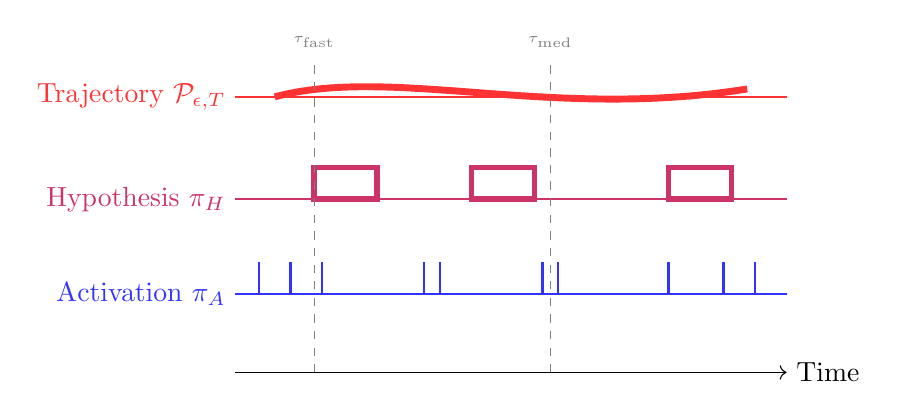
\begin{tikzpicture}[scale=1.0]
  \draw[->] (0,0) -- (7,0) node[right] {Time};

  % Activation layer - fast, many spikes
  \draw[thick, blue!80] (0,1) -- (7,1);
  \foreach \x in {0.3, 0.7, 1.1, 2.4, 2.6, 3.9, 4.1, 5.5, 6.2, 6.6}
    \draw[blue!80, thick] (\x, 1) -- (\x, 1.4);
  \node[left, blue!80] at (0,1) {Activation $\pi_A$};

  % Hypothesis layer - intermediate, fewer features
  \draw[thick, purple!80] (0,2.2) -- (7,2.2);
  \foreach \x in {1.0, 3.0, 5.5}
    \draw[purple!80, thick, line width=2pt] (\x, 2.2) -- (\x+0.8, 2.2) -- (\x+0.8, 2.6) -- (\x, 2.6) -- cycle;
  \node[left, purple!80] at (0,2.2) {Hypothesis $\pi_H$};

  % Trajectory layer - slow, single path
  \draw[thick, red!80] (0,3.5) -- (7,3.5);
  \draw[red!80, thick, line width=2.5pt] (0.5,3.5) .. controls (2,3.9) and (4,3.2) .. (6.5,3.6);
  \node[left, red!80] at (0,3.5) {Trajectory $\mathcal{P}_{\epsilon,T}$};

  % Dashed boundaries indicating timescales
  \draw[dashed, gray] (1,0) -- (1,4) node[above, gray, font=\tiny] {$\tau_{\rm fast}$};
  \draw[dashed, gray] (4,0) -- (4,4) node[above, gray, font=\tiny] {$\tau_{\rm med}$};
\end{tikzpicture}
\caption{Three-timescale stratification of trajectory-induced sparsity. Activation sparsity (blue) operates at fast timescales. Hypothesis tracking (purple) is sparse at intermediate timescales. The admissible trajectory (red) is the slowest and most constrained layer. All three project from a single constrained set $\mathcal{P}_{\epsilon,T}$.}
\label{fig:timescales}
\end{figure}

\section{Thermodynamic Reachability}

The concept of reachability formalizes the constraints on trajectories introduced in the preceding sections. Let $\mathcal{X}$ denote the system's state space and $\mathcal{T} \subseteq \mathcal{X} \times \mathcal{X}$ the set of admissible transitions. Each transition $(x, x') \in \mathcal{T}$ is associated with an energy cost $E(x \to x')$ and a rate constraint determined by the system's capacity to effect the transition within a given time interval.

A trajectory $\{x_t\}_{t=0}^T$ is said to be admissible if it satisfies both the transition and rate constraints at each step. The set of all such trajectories defines the reachable region of $\mathcal{X}$ from an initial state $x_0$. Formally, the reachable set at time $T$ under resource bound $\epsilon$ is defined as
\[
\mathcal{R}_{\epsilon,T}(x_0) = \left\{ x_T \in \mathcal{X} \,\middle|\, \exists \{x_t\}_{t=0}^T \text{ with } x_0 \to x_T, \; (x_t, x_{t+1}) \in \mathcal{T}, \; E(\{x_t\}) \leq \epsilon \right\}.
\]

The hypothesis class available to the system at time $T$ is determined by the set of functions induced by trajectories terminating in $\mathcal{R}_{\epsilon,T}(x_0)$. This class is inherently limited by both the structure of $\mathcal{T}$ and the resource bound $\epsilon$, and it evolves as these quantities change.

An important consequence is that sparsity arises at the level of trajectories rather than representations. Only a small subset of all possible trajectories is admissible, and these trajectories typically involve a limited number of significant transitions. When projected onto the space of representations, this constraint manifests as sparsity in activations and hypotheses.

The following schematic illustrates how $\mathcal{R}_{\epsilon,T}(x_0)$ expands and contracts with available free energy, forming a time-indexed reachable cone rather than a fixed geometric region.

\begin{figure}[h]
\centering
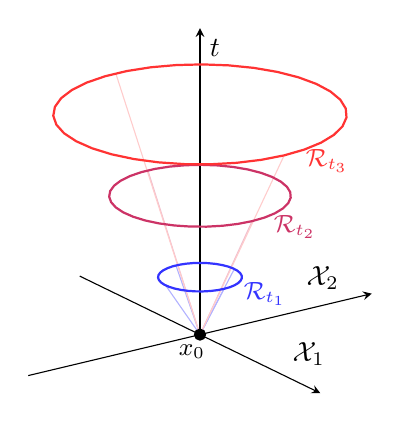
\begin{tikzpicture}[scale=1.0]
\begin{axis}[
    view={55}{25},
    axis lines=center,
    xlabel={$\mathcal{X}_1$}, ylabel={$\mathcal{X}_2$}, zlabel={$t$},
    xtick=\empty, ytick=\empty, ztick=\empty,
    zmin=0, zmax=3.2,
    xmin=-3, xmax=3, ymin=-3, ymax=3,
    width=9cm, height=8cm,
]
  % Cone edge lines
  \addplot3[thin, blue!30] coordinates {(0,0,0) (0.6,0,0.6)};
  \addplot3[thin, blue!30] coordinates {(0,0,0) (-0.6,0,0.6)};
  \addplot3[thin, blue!30] coordinates {(0,0,0) (0,0.6,0.6)};
  \addplot3[thin, blue!30] coordinates {(0,0,0) (0,-0.6,0.6)};
  \addplot3[thin, purple!25] coordinates {(0,0,0) (1.3,0,1.45)};
  \addplot3[thin, purple!25] coordinates {(0,0,0) (-1.3,0,1.45)};
  \addplot3[thin, red!20] coordinates {(0,0,0) (2.1,0,2.3)};
  \addplot3[thin, red!20] coordinates {(0,0,0) (-2.1,0,2.3)};
  % Ring at t1
  \addplot3[thick, blue!80, domain=0:360, samples=36]
    ({0.6*cos(x)}, {0.6*sin(x)}, {0.6});
  \node at (axis cs:0.85,0,0.6) [right, blue!80, font=\small] {$\mathcal{R}_{t_1}$};
  % Ring at t2
  \addplot3[thick, purple!80, domain=0:360, samples=36]
    ({1.3*cos(x)}, {1.3*sin(x)}, {1.45});
  \node at (axis cs:1.6,0,1.45) [right, purple!80, font=\small] {$\mathcal{R}_{t_2}$};
  % Ring at t3
  \addplot3[thick, red!80, domain=0:360, samples=36]
    ({2.1*cos(x)}, {2.1*sin(x)}, {2.3});
  \node at (axis cs:2.4,0,2.3) [right, red!80, font=\small] {$\mathcal{R}_{t_3}$};
  % Origin
  \addplot3[only marks, mark=*, mark size=2pt, black] coordinates {(0,0,0)};
  \node at (axis cs:0.15,0.15,0) [below left, font=\small] {$x_0$};
\end{axis}
\end{tikzpicture}
\caption{Thermodynamic reachability cone $\mathcal{R}_{\epsilon,T}(x_0)$ expanding over time. Each ring marks the boundary of the reachable set at successive times $t_1 < t_2 < t_3$ as free energy accumulates. The cone geometry encodes that reachability is path-dependent and rate-limited, not merely a static ball in state space.}
\label{fig:reachcone}
\end{figure}

The inner ring represents states reachable under minimal energetic conditions. The intermediate ring shows expansion under moderate energy availability. The outer ring corresponds to the broadened hypothesis class accessible when free energy has accumulated sufficiently.

\section{Non-Stationary Hypothesis Classes}

The reachability constraints described above are not static. The system's energetic state, environmental conditions, and prior history all influence the set of admissible transitions and the available resource bound. As a result, the reachable set $\mathcal{R}_{\epsilon,T}(x_0)$ and the induced hypothesis class $\mathcal{H}_{\epsilon,T}$ are time-dependent.

This non-stationarity can be understood in terms of energetic windows. At times when the system has access to greater free energy, either through external input or internal accumulation, it can traverse more complex trajectories and access a broader region of $\mathcal{X}$. Conversely, under energetic stress, the system is restricted to simpler trajectories and a narrower hypothesis class.

Formally, let $\epsilon(t)$ denote the available resource bound at time $t$, and let $\mathcal{T}(t)$ denote the set of admissible transitions under current conditions. The reachable set becomes
\[
\mathcal{R}_{t}(x_0) = \left\{ x_t \in \mathcal{X} \,\middle|\, \exists \{x_\tau\}_{\tau=0}^t \text{ with } (x_\tau, x_{\tau+1}) \in \mathcal{T}(\tau), \; E(\{x_\tau\}) \leq \int_0^t \epsilon(\tau)\, d\tau \right\}.
\]

The corresponding hypothesis class $\mathcal{H}_t$ expands and contracts as $\mathcal{R}_t(x_0)$ changes. Importantly, this evolution is path-dependent. The current state $x_t$ reflects the entire history of prior transitions, and this history determines which future transitions are possible.

This leads to three important consequences. First, inference is path-dependent in a stronger sense than standard Bayesian formulations allow. History does not merely influence beliefs; it determines which belief updates were ever possible. Two systems with identical architectures but different energetic histories can occupy entirely different regions of hypothesis space, even given identical data.

Second, there is no single optimal representation even in principle, because optimality would require access to trajectories that may be energetically unreachable. The system operates within a moving envelope of feasible constructions, and what counts as a good model is always relative to current thermodynamic conditions.

Third, this introduces a natural notion of latent potential: regions of function space that are not currently accessible but could become accessible if the system accumulates sufficient free energy or reorganizes its internal state. The hypothesis space is not merely constrained but conditionally expandable.

The non-stationary nature of the hypothesis class distinguishes this framework from standard models of inference, in which the hypothesis space is fixed and only the distribution over it changes. Here, both the space and the distribution are dynamic, governed by the system's thermodynamic embedding.

\begin{figure}[h]
\centering
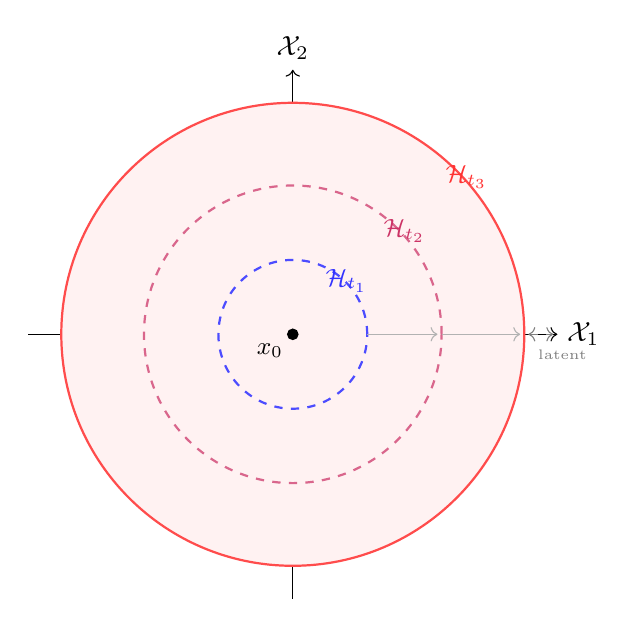
\begin{tikzpicture}[scale=1.05]
  \draw[->] (-3.2,0) -- (3.2,0) node[right] {$\mathcal{X}_1$};
  \draw[->] (0,-3.2) -- (0,3.2) node[above] {$\mathcal{X}_2$};

  % Shaded regions
  \fill[blue!10] (0,0) circle (0.9);
  \fill[purple!8] (0,0) circle (1.8);
  \fill[red!5] (0,0) circle (2.8);

  % Boundaries
  \draw[thick, blue!70, dashed] (0,0) circle (0.9);
  \draw[thick, purple!60, dashed] (0,0) circle (1.8);
  \draw[thick, red!70] (0,0) circle (2.8);

  % Labels
  \node[blue!80, font=\small] at (0.65, 0.65) {$\mathcal{H}_{t_1}$};
  \node[purple!80, font=\small] at (1.35, 1.25) {$\mathcal{H}_{t_2}$};
  \node[red!80, font=\small] at (2.1, 1.9) {$\mathcal{H}_{t_3}$};

  % Latent region annotation
  \draw[<->, gray, dashed] (2.85,0) -- (3.15,0);
  \node[gray, font=\tiny, right] at (2.85,-0.25) {latent};

  % Origin
  \filldraw[black] (0,0) circle (1.8pt) node[below left, font=\small] {$x_0$};

  % Arrows showing expansion
  \draw[->, gray!60] (0.9,0) -- (1.75,0);
  \draw[->, gray!60] (1.8,0) -- (2.75,0);
\end{tikzpicture}
\caption{Non-stationary hypothesis class $\mathcal{H}_t$ expanding with available free energy. The innermost region (blue) is accessible at low energy $t_1$; the middle ring (purple) opens at $t_2$ as energy accumulates; the outer region (red) represents hypotheses accessible only at $t_3$. The region beyond $\mathcal{H}_{t_3}$ marks latent potential: structurally present but not yet energetically reachable.}
\label{fig:nonstationary}
\end{figure}

\section{Formal Correspondences: RSVP and Spherepop}

The trajectory-based framework developed above admits natural correspondences with existing formalisms that emphasize dynamical structure and irreversibility. Two such formalisms are the Relativistic Scalar-Vector Plenum (RSVP) framework and the Spherepop calculus.

In the RSVP framework, the system is described by scalar, vector, and entropy fields, denoted $\Phi(x,t)$, $\mathbf{v}(x,t)$, and $S(x,t)$, respectively. These fields define the local geometry of state space and the dynamics of transitions. The scalar field $\Phi$ encodes potential structure, the vector field $\mathbf{v}$ encodes directional flow, and the entropy field $S$ modulates the cost and admissibility of transitions.

Within this framework, thermodynamic reachability corresponds to flow constrained by the fields $(\Phi, \mathbf{v}, S)$. Regions of high entropy or steep gradients impose higher transition costs, effectively restricting the set of admissible trajectories. The non-stationarity of the hypothesis class is captured by the time dependence of these fields, which evolve in response to both internal dynamics and environmental interactions. Inference is thereby recast as field-constrained flow: the admissible trajectory manifold is itself a dynamical object, continuously reshaped by $S(x,t)$.

The Spherepop calculus provides a complementary perspective based on irreversible event histories. In this formalism, the state of a system is represented by a history $H_t$ of discrete events, and transitions correspond to the addition of new events to this history. The identity of the system is defined by its history, and there is no mechanism for reversing or erasing events.

From the perspective of thermodynamic reachability, Spherepop can be interpreted as a discrete analogue of trajectory construction. Each admissible transition corresponds to an event appended to the history, and the set of possible futures is determined by which events are energetically realizable at a given time. Branches that are not realized are not explicitly pruned; they simply never enter the history due to constraint. Identity-as-history is therefore inseparable from identity-as-reachability: the system's trajectory is constitutive of what it is.

Together, these correspondences illustrate that the trajectory-based framework is not tied to a particular mathematical representation, but reflects a more general structure in which dynamics, constraint, and history are inseparable.

\section{Non-Invertibility of Compressed Trust Representations}

The evaluation of trust as a functional on histories introduces a structural asymmetry between full histories and their compressed representations.

Let $\mathcal{H}$ denote the space of construction histories and $\mathcal{T} : \mathcal{H} \to [0,1]$ a trust functional. Let $\phi : \mathcal{H} \to \mathcal{C}$ be a compression mapping into a lower-dimensional space $\mathcal{C}$.

\begin{lemma}[Non-Invertibility of Trust Under Compression]
If $\phi$ is lossy, that is, not injective, then in general there does not exist a function $\tilde{\mathcal{T}} : \mathcal{C} \to [0,1]$ such that $\tilde{\mathcal{T}}(\phi(H)) = \mathcal{T}(H)$ for all $H \in \mathcal{H}$.
\end{lemma}

\begin{proof}
Since $\phi$ is not injective, there exist $H_1 \neq H_2$ such that $\phi(H_1) = \phi(H_2)$. If $\mathcal{T}(H_1) \neq \mathcal{T}(H_2)$, then no function $\tilde{\mathcal{T}}$ defined on $\mathcal{C}$ can distinguish between them. Therefore, $\mathcal{T}$ cannot be recovered from $\phi(H)$ in general.
\end{proof}

This establishes that compression schemes replacing histories with tokens necessarily discard information required for trust evaluation. The connection to thermodynamic reachability is direct. Just as physical constraints limit which histories can be constructed, epistemic constraints limit which histories can be evaluated and trusted. Both are governed by the structure of trajectories, and both are susceptible to distortion under compression. When histories are compressed into reputational markers, certifications, or symbolic tokens, the non-invertibility of $\phi$ ensures that failures are both inevitable and non-recoverable without the original construction record.

\section{Transition to Externalized Constraint Structures}

The preceding sections establish that both inference and trust depend fundamentally on the structure of trajectories. Internal state evolution is restricted by thermodynamic reachability, and epistemic evaluation depends on access to construction history. Both results converge on a common structural principle: constraint systems define the space of admissible transformations, and projections of those transformations introduce loss.

This principle does not apply exclusively to internal processes. Any structure that encodes transformation rules and can be engaged by a system participates in the same constraint geometry. External symbolic artifacts, including mathematical formulas, formal systems, and human-generated outputs, therefore admit a natural reinterpretation as externalized constraint operators. The next section develops this extension.

\section{Externalized Formal Systems as Constraint Operators}

A mathematical formula can be understood as a compact encoding of a transformation rule acting on a space of admissible inputs. Let $F : \mathcal{X} \to \mathcal{X}$ denote such a mapping. While $F$ may be finitely specified, its evaluation can generate outputs of arbitrarily high complexity, often exceeding the immediate computational capacity of the system that applies it. Recursive or iterative definitions induce behaviors not trivially predictable from their defining expressions.

Let $\mathcal{F}$ denote a set of such operators. When a system applies $F \in \mathcal{F}$ to a state $x \in \mathcal{X}$, it undergoes a transition
\[
(x, F) \mapsto x' = F(x),
\]
which may involve a sequence of internal computations required to evaluate $F$. The cost of this transition depends not only on the complexity of $F$ but also on the system's capacity to realize the transformation under its energetic and rate constraints.

Let $\mathcal{T}_{int}$ denote the set of admissible internal transitions and $\mathcal{T}_{ext}$ the set of transitions induced by applying operators in $\mathcal{F}$. The combined transition set
\[
\mathcal{T}' = \mathcal{T}_{int} \cup \mathcal{T}_{ext}
\]
defines an augmented reachability structure. This expansion is itself constrained: the system must still evaluate $F$ under its energetic and temporal limitations, and thus only a subset of $\mathcal{F}$ is effectively usable at any given time.

The unpredictability associated with formal operators arises from their role as compressed representations of complex processes. While the defining expression of $F$ may be simple, the space of possible outputs under variation of inputs or iterative application can be large and structurally rich. This mirrors the behavior of admissible trajectories in $\mathcal{P}_{\epsilon,T}$, where simple local rules generate complex global structure.

Human-generated artifacts, including artworks and symbolic constructions, admit the same interpretation. Each artifact encodes a transformation on the internal state of a system interacting with it. When engaged, it induces a trajectory reflecting the structure embedded in the artifact. The artifact does not possess agency in a psychological sense, but functions as a constraint operator that shapes state evolution.

This interpretation aligns with the earlier analysis of trust and compression. Just as internal trajectories define the identity of a system's representations, the structure of an external operator determines the transformations it can induce. When such operators are treated as opaque tokens rather than explicit structures, the same non-invertibility issues arise, and their effective role in shaping trajectories becomes inaccessible.

The key result is that external formal systems are not merely representations but active components of the system's constraint geometry. They extend the space of admissible trajectories while remaining subject to the same principles of reachability, rate limitation, and history dependence. Internal inference and external symbolic interaction are thereby unified as instances of constrained trajectory construction, governed by the same underlying principles.

\section{Implications for Machine Learning and Artificial Systems}

The framework developed in this work has several implications for the design and analysis of machine learning systems. Most contemporary models assume a fixed architecture and hypothesis space, with regularization techniques used to control complexity. This contrasts with the dynamic, constraint-driven hypothesis classes described here.

Incorporating thermodynamic principles into artificial systems suggests the development of architectures in which the effective hypothesis class evolves over time, conditioned on resource availability and system history. Rather than imposing sparsity through penalties, such systems would exhibit sparsity as a consequence of limited computational and energetic resources.

This perspective also highlights the importance of path dependence in learning. Systems that explicitly track their construction history may be better able to adapt to changing conditions and avoid catastrophic failures associated with compressed representations. Conversely, systems that rely heavily on lossy compression may exhibit brittle behavior when confronted with scenarios requiring reconstruction of underlying processes.

\section{Philosophical Return: Knowledge as Reachable Construction}

The formal developments of this work support a broader epistemological claim: knowledge is not a static property of representations, but a consequence of reachable construction. A representation is meaningful only insofar as it can be constructed through admissible trajectories, and its validity depends on the integrity of its construction history.

This perspective challenges the notion that trust can be assigned to objects independently of their history. Instead, trust is a functional defined over construction histories, and the non-invertibility established in Section~12 guarantees that no compression of those histories can preserve the full structure of trust evaluation. Maintaining explicit histories preserves invertibility and allows trust to be derived from structural properties rather than assigned as an external label.

This epistemological result mirrors the physical one. Just as thermodynamic reachability determines which trajectories can be constructed, epistemic constraints determine which of those trajectories can be evaluated and trusted. Both processes are governed by the structure of histories, and both are susceptible to distortion under compression.

\section{Entropy of Transition Across Topological Boundaries}

The non-stationary nature of the reachability manifold implies that transitions may occur in which the topology of the admissible trajectory space changes. Such transitions correspond to bifurcations in the scalar potential $\Phi(x,t)$ or degeneracies in the reachability metric $g_{\mu\nu}$, resulting in a restructuring of the accessible hypothesis class.

Let $\mathcal{M}_-$ and $\mathcal{M}_+$ denote the reachability manifolds immediately before and after a topological transition at time $t = t_c$. Let $\mathcal{P}_-$ and $\mathcal{P}_+$ denote the corresponding sets of admissible trajectories, and let $\mathcal{H}_-$ and $\mathcal{H}_+$ be the induced hypothesis classes.

In general, there does not exist a bijective mapping between $\mathcal{P}_-$ and $\mathcal{P}_+$. Certain trajectories admissible in $\mathcal{M}_-$ may become unreachable in $\mathcal{M}_+$, and new trajectories may become available. This induces a loss of reconstructible construction history.

\begin{definition}[Entropy of Transition]
Let $\mu_-$ be a measure over $\mathcal{P}_-$ induced by trajectory costs, and let $\pi : \mathcal{P}_- \to \mathcal{P}_+$ be the projection mapping induced by the topological transition, where undefined mappings correspond to trajectories that are no longer admissible. The entropy of transition is defined as
\[
\Delta S_{\mathrm{trans}} = - \int_{\mathcal{P}_-} \mu_-(\gamma) \log \left( \frac{\mu_+(\pi(\gamma))}{\mu_-(\gamma)} \right) d\gamma,
\]
where $\mu_+$ is the induced measure on $\mathcal{P}_+$.
\end{definition}

\begin{remark}
The quantity $\Delta S_{\mathrm{trans}}$ measures the divergence between the pre-transition and post-transition trajectory distributions. It captures the extent to which construction histories lose correspondence under the new reachability geometry.
\end{remark}

\begin{proposition}[Irreducible Information Loss]
If the transition from $\mathcal{M}_-$ to $\mathcal{M}_+$ is topologically non-trivial, then $\Delta S_{\mathrm{trans}} > 0$.
\end{proposition}

\begin{proof}[Sketch]
A topological change implies that there exist trajectories in $\mathcal{P}_-$ with no admissible image under $\pi$, or multiple trajectories mapping to the same image. In either case, the mapping is non-invertible. This induces a strictly positive divergence between $\mu_-$ and the pushforward measure $\pi_* \mu_-$, implying $\Delta S_{\mathrm{trans}} > 0$.
\end{proof}

This result formalizes the intuitive notion that paradigm shifts incur irreversible information loss. Even though the system's history $H$ remains intact as a record, its projection into the new hypothesis class $\mathcal{H}_+$ is no longer injective. Portions of the history become non-reconstructible within the new reachability structure.

\subsection{Trust Renormalization Across Transitions}

Let $\mathcal{T}(H)$ be the trust functional defined over histories. Following a topological transition, the effective trust must be renormalized to account for the loss of reconstructibility. Define the preserved history subset
\[
H_{\mathrm{pres}} = \{ h \in H \mid h \text{ remains admissible under } \mathcal{M}_+ \}.
\]
Then the renormalized trust functional is given by
\[
\mathcal{T}_+(H) = \mathcal{T}(H_{\mathrm{pres}}),
\]
with the residual contribution of non-admissible history components decaying as a function of $\Delta S_{\mathrm{trans}}$.

\begin{remark}
In the limit where $\Delta S_{\mathrm{trans}}$ is large, the overlap between $\mathcal{P}_-$ and $\mathcal{P}_+$ vanishes, and $\mathcal{T}_+(H) \to 0$. This corresponds to an epistemic discontinuity in which prior construction history no longer supports trust evaluation.
\end{remark}

\subsection{Geometric Interpretation}

From a geometric perspective, the entropy of transition quantifies the change in volume and curvature of the reachability manifold. Regions of $\mathcal{M}_-$ that collapse or bifurcate under the transition contribute positively to $\Delta S_{\mathrm{trans}}$, reflecting the loss of accessible trajectories. In the RSVP correspondence, this corresponds to regions where gradients of the entropy field $S(x,t)$ induce degeneracies in the metric $g_{\mu\nu}$. In the Spherepop formalism, it corresponds to segments of the event history that remain recorded but are no longer traversable under the updated constraint structure. Thus, $\Delta S_{\mathrm{trans}}$ provides a unifying quantity that links thermodynamic irreversibility, geometric restructuring, and epistemic discontinuity.

\begin{figure}[h]
\centering
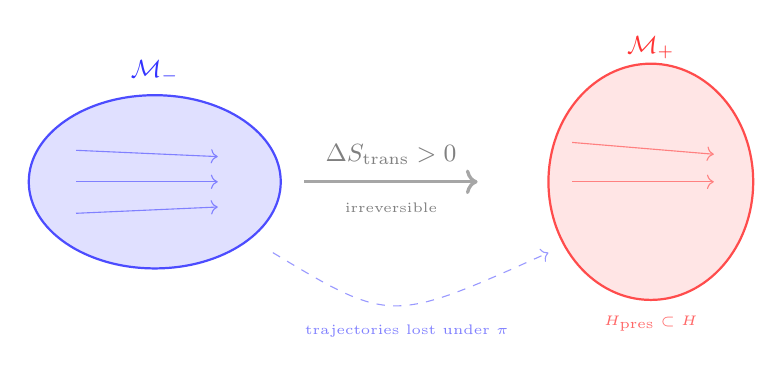
\begin{tikzpicture}[scale=1.0]
  % Pre-transition manifold M_-
  \fill[blue!12] (-3.5,0) ellipse (1.6 and 1.1);
  \draw[thick, blue!70] (-3.5,0) ellipse (1.6 and 1.1);
  \node[blue!80, font=\small] at (-3.5, 1.4) {$\mathcal{M}_-$};

  % Some sample trajectories inside M_-
  \foreach \dy in {-0.4, 0, 0.4}
    \draw[blue!50, ->] (-4.5, \dy) -- (-2.7, \dy*0.8);

  % Transition arrow with Delta S label
  \draw[->, very thick, gray!70] (-1.6,0) -- (0.6,0);
  \node[above, gray, font=\small] at (-0.5, 0.1) {$\Delta S_{\mathrm{trans}} > 0$};
  \node[below, gray, font=\tiny] at (-0.5, -0.15) {irreversible};

  % Post-transition manifold M_+
  \fill[red!10] (2.8,0) ellipse (1.3 and 1.5);
  \draw[thick, red!70] (2.8,0) ellipse (1.3 and 1.5);
  \node[red!80, font=\small] at (2.8, 1.7) {$\mathcal{M}_+$};

  % Fewer trajectories in M_+ (some lost)
  \foreach \dy in {0, 0.5}
    \draw[red!50, ->] (1.8, \dy) -- (3.6, \dy*0.7);

  % Lost trajectories annotation
  \draw[blue!40, dashed, ->] (-2.0,-0.9) .. controls (-0.5,-1.8) .. (1.5,-0.9);
  \node[blue!50, font=\tiny] at (-0.3,-1.9) {trajectories lost under $\pi$};

  % H_pres label
  \node[red!60, font=\tiny] at (2.8,-1.8) {$H_{\mathrm{pres}} \subset H$};
\end{tikzpicture}
\caption{Topological transition from $\mathcal{M}_-$ to $\mathcal{M}_+$. Trajectories admissible under $\mathcal{M}_-$ (blue arrows) that have no image under the projection $\pi$ are lost, contributing to $\Delta S_{\mathrm{trans}} > 0$. The preserved history $H_{\mathrm{pres}}$ is the subset of pre-transition construction history that remains admissible under the new reachability structure.}
\label{fig:topology}
\end{figure}

\section{Continuous-Time Reachability and an Action Functional}

The discrete formulation of reachability can be extended to a continuous-time setting in order to make the geometry of thermodynamic constraints more explicit. Let the state space remain $\mathcal{X} = \mathbb{R}^n$, and let a trajectory be a continuously differentiable curve $x : [0,T] \to \mathcal{X}$ evolving under controlled dynamics $\dot{x}(t) = u(t)$ for a time-dependent control input $u(t) \in \mathbb{R}^n$. The thermodynamic cost of a trajectory is modeled by a Lagrangian
\[
\mathcal{L}(x,\dot{x},t) = \tfrac{1}{2}\|\dot{x}(t)\|^2 + V(x(t),t),
\]
where the kinetic term captures transition expenditure and $V(x,t)$ represents environmental or internal constraint geometry. The action associated with a trajectory is
\[
\mathcal{S}[x] = \int_0^T \mathcal{L}(x,\dot{x},t)\,dt.
\]
A trajectory is thermodynamically admissible if $\mathcal{S}[x] \leq \Lambda(T)$, where $\Lambda(T)$ is the total available energetic budget. The continuous-time reachable set is therefore
\[
\mathcal{R}_{\Lambda,T}(x_0) = \left\{ x(T) \;\middle|\; x(0)=x_0,\; \mathcal{S}[x]\leq \Lambda(T) \right\}.
\]
This formulation makes explicit that reachability depends not only on endpoints but on the full path connecting them.

\subsection{Euler--Lagrange Structure}

Among admissible trajectories, those minimizing the action satisfy the Euler--Lagrange equations, which in the present case reduce to
\[
\ddot{x}^i(t) + \frac{\partial V}{\partial x^i}(x(t),t) = 0.
\]
These describe geodesic-like flow through the constrained state space. Inference, under this formulation, is no longer a search over a fixed hypothesis set but a variational problem over admissible histories.

\subsection{Time-Dependent Energy Windows}

If the available energy varies in time, the admissibility bound becomes $\mathcal{S}[x] \leq \int_0^T \lambda(t)\,dt$ for an instantaneous energy-availability function $\lambda(t)$. The reachable set then becomes explicitly non-stationary:
\[
\mathcal{R}_{T}(x_0) = \left\{ x(T) \;\middle|\; x(0)=x_0,\; \mathcal{S}[x]\leq \int_0^T \lambda(t)\,dt \right\}.
\]
A path admissible during one energetic window may be inaccessible during another, even if the background geometry $V(x,t)$ remains unchanged.

\subsection{Trajectory Sparsity in the Continuous Setting}

Sparsity in the continuous setting appears as concentration of action along a restricted subset of directions in tangent space. If admissible trajectories minimizing $\mathcal{S}[x]$ lie predominantly in a low-dimensional distribution $\mathcal{D}_x \subset T_x\mathcal{X}$ with $\dim \mathcal{D}_x \ll n$, then the system exhibits trajectory sparsity. Apparent sparsity in activations or maintained hypotheses is a projection of this deeper restriction on admissible motion.

\subsection{Induced Continuous-Time Hypothesis Class}

Let a hypothesis be a functional of the terminal state or of the full trajectory. The effective hypothesis class is
\[
\mathcal{H}_{\Lambda,T} = \left\{ h \;\middle|\; h \text{ is induced by some admissible trajectory } x(\cdot) \right\}.
\]
Because admissibility depends on the action bound $\Lambda(T)$ and the constraint landscape $V(x,t)$, the hypothesis class is not fixed. It is a dynamically evolving consequence of physically realizable histories. This provides a direct bridge between thermodynamic embedding and geometric inference: a system's effective inferential capacity is the set of trajectory functionals realizable under its action budget.

\begin{figure}[h]
\centering
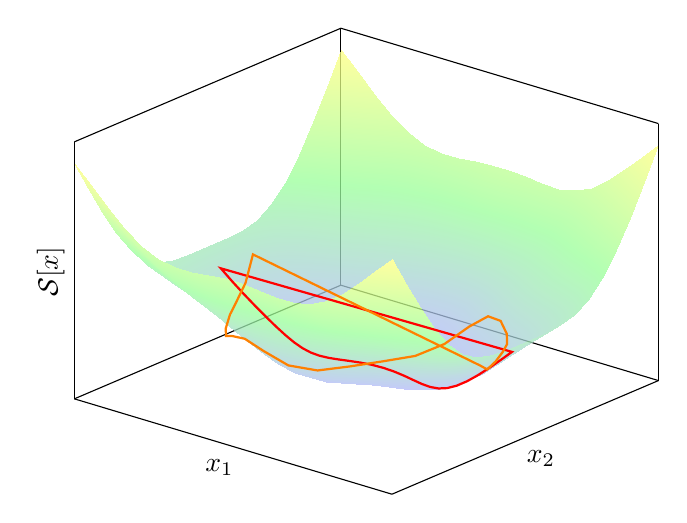
\begin{tikzpicture}
\begin{axis}[
    view={40}{30},
    xlabel={$x_1$}, ylabel={$x_2$}, zlabel={$\mathcal{S}[x]$},
    samples=20, domain=-2:2, y domain=-2:2,
    width=9cm, height=7.5cm,
    xtick=\empty, ytick=\empty, ztick=\empty,
    colormap={greenblue}{color=(blue!30) color=(green!40) color=(yellow!50)},
]
  % Action landscape surface
  \addplot3[surf, shader=interp, opacity=0.75]
    {0.6*x^2 + 1.2*y^2 + 0.3*cos(deg(3*x))*cos(deg(3*y))};

  % Minimum-action trajectory (red curve along x-axis valley)
  \addplot3[thick, red, domain=-1.8:1.8, samples=30]
    ({x}, {0.05*sin(deg(4*x))}, {0.6*x^2 + 0.3*cos(deg(3*x))});

  % Inadmissible high-cost path (dashed orange)
  \addplot3[thick, orange, dashed, domain=-1.8:1.8, samples=24]
    ({x}, {1.0*sin(deg(2*x))}, {0.6*x^2 + 1.2*(sin(deg(2*x)))^2 + 0.3*cos(deg(3*x))*cos(deg(6*x))});
\end{axis}
\end{tikzpicture}
\caption{Action landscape $\mathcal{S}[x]$ over state space. The red curve is the minimum-action trajectory satisfying the Euler--Lagrange equations; this is the geodesic recovered in the saddle-point limit $\beta \to \infty$. The dashed orange curve represents a higher-cost path that may fall outside the admissible set $\Gamma_\Lambda$ under tight energetic constraints.}
\label{fig:actionlandscape}
\end{figure}

\section{A Partition Function Over Admissible Trajectories}

The variational formulation admits a statistical extension in which inference is interpreted as a weighted ensemble over admissible trajectories rather than a single optimal path. Let $\Gamma(x_0,T)$ denote the set of trajectories with $x(0)=x_0$ over $[0,T]$, and define the admissible ensemble
\[
\Gamma_{\Lambda}(x_0,T) = \left\{ x(\cdot)\in\Gamma(x_0,T) \;\middle|\; \mathcal{S}[x]\leq \Lambda(T) \right\}.
\]
The partition function over admissible trajectories is
\[
Z(x_0,T) = \int_{\Gamma_{\Lambda}(x_0,T)} e^{-\beta \mathcal{S}[x]} \,\mathcal{D}x,
\]
where $\beta > 0$ is an inverse resource parameter and $\mathcal{D}x$ denotes the formal measure over trajectories. The induced probability density over admissible trajectories is
\[
P[x \mid x_0,T] = \frac{1}{Z(x_0,T)} e^{-\beta \mathcal{S}[x]} \mathbf{1}_{\{\mathcal{S}[x]\leq \Lambda(T)\}}.
\]
There is no independently encoded prior over hypotheses. Lower-action trajectories receive greater weight because they are more thermodynamically accessible, and the effective prior is the measure induced by the action landscape and admissibility bound.

\subsection{Bayesian Interpretation}

If observational data $D$ constrain trajectories through a mismatch functional $\mathcal{L}_D[x]$, the posterior measure is
\[
P[x \mid D, x_0,T] \propto e^{-\beta \mathcal{S}[x] - \alpha \mathcal{L}_D[x]} \mathbf{1}_{\{\mathcal{S}[x]\leq \Lambda(T)\}},
\]
with posterior partition function
\[
Z_D(x_0,T) = \int_{\Gamma_{\Lambda}(x_0,T)} e^{-\beta \mathcal{S}[x] - \alpha \mathcal{L}_D[x]} \,\mathcal{D}x.
\]
This yields a path-integral Bayesianism: the system updates over physically admissible histories, not abstract hypotheses.

\subsection{Free Energy and Reachability}

The partition function induces an effective free energy
\[
\mathcal{F}(x_0,T) = -\frac{1}{\beta}\log Z(x_0,T).
\]
A lower free energy corresponds to a larger or more cheaply reachable set of trajectories, while a higher free energy indicates a narrower inferential envelope. Thermodynamic reachability and Bayesian updating are thereby formally linked: both are governed by the weighted structure of admissible histories.

\subsection{Saddle-Point Limit and Recovery of Variational Flow}

The partition-function and variational formulations are related by regime rather than by contradiction. In the limit of strong energetic discrimination, the ensemble concentrates around action-minimizing paths.

\begin{proposition}[Saddle-Point Recovery of Variational Trajectories]
Let $Z(x_0,T)$ be the partition function over admissible trajectories, and assume that $\mathcal{S}[x]$ admits a finite set of smooth local minima $\{x^\ast_k(\cdot)\}$ in $\Gamma_{\Lambda}(x_0,T)$. Then, in the limit $\beta \to \infty$, the dominant contribution to $Z(x_0,T)$ comes from the action-minimizing trajectories. If the minimizer is unique, then
\[
P[x \mid x_0,T] \to \delta[x-x^\ast] \qquad \text{as } \beta \to \infty,
\]
where $x^\ast(\cdot)$ satisfies the Euler--Lagrange equations associated with $\mathcal{S}[x]$.
\end{proposition}

\begin{proof}[Sketch]
As $\beta \to \infty$, trajectories with action strictly greater than the minimum are exponentially suppressed. A saddle-point approximation yields
\[
Z(x_0,T) \sim \sum_k e^{-\beta \mathcal{S}[x^\ast_k]} \left(\det \mathcal{H}_k\right)^{-1/2},
\]
where $\mathcal{H}_k$ is the Hessian of the action at $x^\ast_k$. If the minimizer is unique, the normalized measure concentrates on that trajectory, and since extrema of $\mathcal{S}[x]$ satisfy the Euler--Lagrange equations, the limiting trajectory is variationally admissible.
\end{proof}

\begin{remark}
The parameter $\beta$ controls the concentration of inferential weight. Small $\beta$ corresponds to a broad exploratory regime. Large $\beta$ recovers geometric flow as the zero-temperature limit of the statistical formulation.
\end{remark}

\begin{corollary}[Recovery of Action-Bounded Bayesian Flow]
In the joint saddle-point limit of $Z_D(x_0,T)$, the posterior measure concentrates on trajectories minimizing the effective action
\[
\mathcal{S}_{\mathrm{eff}}[x] = \mathcal{S}[x] + \frac{\alpha}{\beta}\mathcal{L}_D[x].
\]
Consequently, posterior inference reduces to variational flow on the effective constraint landscape, and observational updating is realized as a deformation of the reachability geometry rather than reweighting over a fixed hypothesis set.
\end{corollary}

\begin{figure}[h]
\centering
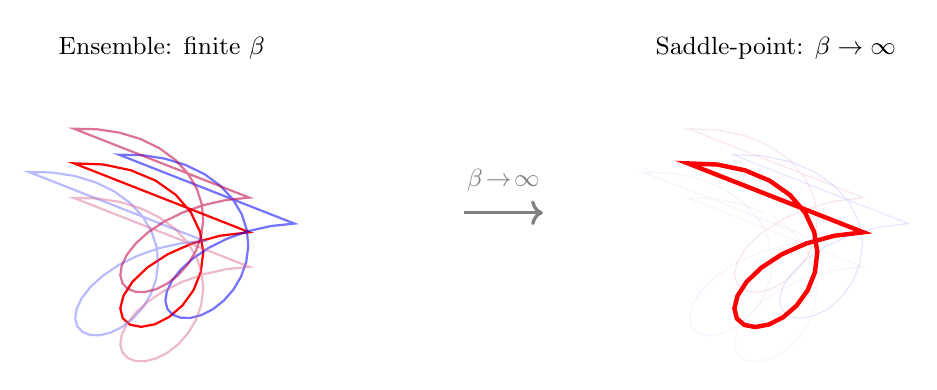
\begin{tikzpicture}[scale=1.0]
  % LEFT PANEL: ensemble at finite beta
  \begin{scope}[xshift=0cm]
    \begin{axis}[
        view={55}{20}, axis lines=none,
        width=7cm, height=6cm,
        title={\small Ensemble: finite $\beta$},
        title style={font=\small},
    ]
      \addplot3[thick, red, domain=0:6.28, samples=24]
        ({x/2}, {sin(deg(x))*0.5}, {cos(deg(x))*0.5});
      \addplot3[thick, blue, opacity=0.55, domain=0:6.28, samples=30]
        ({x/2}, {sin(deg(x))*0.5+0.28}, {cos(deg(x))*0.5});
      \addplot3[thick, blue!60, opacity=0.45, domain=0:6.28, samples=30]
        ({x/2}, {sin(deg(x))*0.5-0.28}, {cos(deg(x))*0.5});
      \addplot3[thick, purple, opacity=0.55, domain=0:6.28, samples=30]
        ({x/2}, {sin(deg(x))*0.5}, {cos(deg(x))*0.5+0.28});
      \addplot3[thick, purple!60, opacity=0.45, domain=0:6.28, samples=30]
        ({x/2}, {sin(deg(x))*0.5}, {cos(deg(x))*0.5-0.28});
    \end{axis}
  \end{scope}
  % Arrow
  \draw[->, very thick, gray] (6.55,2.8) -- (7.55,2.8);
  \node[above, gray, font=\small] at (7.05,2.95) {$\beta\!\to\!\infty$};
  % RIGHT PANEL: saddle-point collapse
  \begin{scope}[xshift=7.8cm]
    \begin{axis}[
        view={55}{20}, axis lines=none,
        width=7cm, height=6cm,
        title={\small Saddle-point: $\beta \to \infty$},
        title style={font=\small},
    ]
      \addplot3[ultra thick, red, domain=0:6.28, samples=24]
        ({x/2}, {sin(deg(x))*0.5}, {cos(deg(x))*0.5});
      \addplot3[blue, opacity=0.10, domain=0:6.28, samples=24]
        ({x/2}, {sin(deg(x))*0.5+0.28}, {cos(deg(x))*0.5});
      \addplot3[blue!60, opacity=0.08, domain=0:6.28, samples=24]
        ({x/2}, {sin(deg(x))*0.5-0.28}, {cos(deg(x))*0.5});
      \addplot3[purple, opacity=0.10, domain=0:6.28, samples=24]
        ({x/2}, {sin(deg(x))*0.5}, {cos(deg(x))*0.5+0.28});
      \addplot3[purple!60, opacity=0.08, domain=0:6.28, samples=24]
        ({x/2}, {sin(deg(x))*0.5}, {cos(deg(x))*0.5-0.28});
    \end{axis}
  \end{scope}
\end{tikzpicture}
\caption{Left: trajectory ensemble at finite $\beta$. Multiple admissible paths (blue, purple) contribute to the partition function $Z(x_0,T)$, weighted by $e^{-\beta\mathcal{S}[x]}$. Right: saddle-point limit $\beta \to \infty$. The measure collapses onto the action-minimizing trajectory (red, bold), recovering variational geometric flow. All other paths are exponentially suppressed.}
\label{fig:ensemble}
\end{figure}

\section{Closed-Loop Optimization and the Projection Trap}

\subsection{Empirical Overperformance and Generalization Failure}

A recurring phenomenon across machine learning, finance, and adaptive systems is the appearance of strong performance under controlled or historical conditions, followed by rapid degradation upon deployment. This is commonly described in terms of overfitting, distributional shift, or in-sample versus out-of-sample failure. However, these terms often obscure a deeper structural issue: the system has not learned the generative process, but rather a projection of it.

Let $\mathcal{D}_n = \{x_i\}_{i=1}^n$ denote a finite dataset sampled from an underlying process $\mathcal{P}$. Any learning procedure constructs a hypothesis $h \in \mathcal{H}$ that minimizes empirical risk
\[
\mathcal{L}_{\mathcal{D}_n}(h) = \frac{1}{n} \sum_{i=1}^n \ell(h(x_i)).
\]
This objective is necessarily defined over $\mathcal{D}_n$, not over $\mathcal{P}$ itself. The hypothesis therefore aligns with the statistical structure of the dataset, which is only a finite projection of the full process. The dataset encodes a particular realization of $\mathcal{P}$, containing contingent correlations, sampling artifacts, and finite-resolution structure. The learned model, in minimizing empirical loss, captures this projection. It does not, in general, recover the generative mechanism that produced it.

\subsection{The Projection Gap}

We formalize this discrepancy as the \emph{projection gap}. Let $\mathcal{R}_{\mathcal{P}}(h)$ denote the true risk under the generative process and $\mathcal{R}_{\mathcal{D}_n}(h)$ the empirical risk. Then
\[
\Delta_{\mathrm{proj}}(h) = \left| \mathcal{R}_{\mathcal{P}}(h) - \mathcal{R}_{\mathcal{D}_n}(h) \right|
\]
measures the extent to which performance on the dataset fails to reflect performance under the process. As $n$ increases, $\mathcal{D}_n$ refines the projection of $\mathcal{P}$, but does not converge to it in any constructive sense unless strong assumptions are imposed. This leads to an important asymmetry: increasing dataset size reduces variance within the projection but does not eliminate the structural mismatch between projection and process. The model may become increasingly confident while remaining systematically misaligned with the generative dynamics.

\subsection{Closed-Loop Optimization}

The projection gap becomes pathological under repeated optimization. Consider an iterative procedure that updates $h_t$ to minimize empirical loss on a fixed dataset $\mathcal{D}_n$:
\[
h_{t+1} = \arg\min_{h \in \mathcal{H}} \mathcal{L}_{\mathcal{D}_n}(h \mid h_t).
\]
As $t \to \infty$, the optimization process exhausts the signal present in $\mathcal{D}_n$ and begins to exploit its idiosyncratic structure. The hypothesis increasingly encodes dataset-specific artifacts rather than features of $\mathcal{P}$. This defines the \emph{closed-loop optimization trap}: improvement with respect to $\mathcal{D}_n$ no longer corresponds to improvement with respect to $\mathcal{P}$.

\begin{proposition}[Closed-Loop Divergence]
For sufficiently expressive $\mathcal{H}$, there exists a sequence $\{h_t\}$ such that
\[
\lim_{t \to \infty} \mathcal{R}_{\mathcal{D}_n}(h_t) = 0 \quad \text{while} \quad \mathcal{R}_{\mathcal{P}}(h_t) \not\to 0.
\]
\end{proposition}

\begin{proof}[Sketch]
Given a finite dataset $\mathcal{D}_n$, an expressive hypothesis class can represent functions that interpolate the dataset exactly, achieving zero empirical risk. Since $\mathcal{P}$ generates samples outside the support of $\mathcal{D}_n$ with nonzero probability, the true risk remains bounded away from zero.
\end{proof}

\subsection{Goodhart Effects and Metric Collapse}

This phenomenon is closely related to Goodhart's Law: when a measure becomes a target, it ceases to be a good measure. Let $\phi: \mathcal{H} \to \mathbb{R}$ be a proxy metric and $\psi: \mathcal{H} \to \mathbb{R}$ the true objective. If $\phi$ is not injective with respect to $\psi$, then there exist $h_1, h_2$ such that
\[
\phi(h_1) = \phi(h_2) \quad \text{but} \quad \psi(h_1) \neq \psi(h_2).
\]
Optimization over $\phi$ alone cannot distinguish between such hypotheses, allowing divergence from the true objective.

\subsection{Kolmogorov Perspective}

The projection gap admits an information-theoretic interpretation. Let $K(\mathcal{P})$ denote the Kolmogorov complexity of the generative process. For most real-world processes, $K(\mathcal{P})$ is effectively unbounded relative to any finite dataset description, so any model $h$ constructed from $\mathcal{D}_n$ is a lossy compression: $K(h) \ll K(\mathcal{P})$. The compression error concentrates in regions of the input space not represented in $\mathcal{D}_n$, which is precisely where deployment occurs. Generalization failure is not accidental but necessary: it is the manifestation of irreducible compression loss when a finite representation approximates an effectively incompressible process.

\section{Derivation of the Projection Trap from Thermodynamic Reachability}

The account of closed-loop optimization can be derived directly from the reachability formalism. A finite dataset does not merely provide examples; it induces a restricted submanifold of admissible inferential motion, and optimization over that dataset takes place within a compressed region of trajectory space.

Let $\mathcal{P}$ denote the underlying generative process and $\mathcal{D}_n$ a finite sample. Associated to $\mathcal{D}_n$ is a restricted transition structure $\mathcal{T}_{\mathcal{D}_n} \subseteq \mathcal{T}_{\mathcal{P}}$, where $\mathcal{T}_{\mathcal{P}}$ is the full set of admissible transitions induced by the generative environment. This induces a dataset-restricted reachable set
\[
\mathcal{R}_{\mathcal{D}_n,\epsilon,T}(x_0) = \left\{ x_T \in \mathcal{X} \;\middle|\; \exists \{x_t\}_{t=0}^T \text{ with } (x_t,x_{t+1}) \in \mathcal{T}_{\mathcal{D}_n},\; E(\{x_t\}) \le \epsilon \right\},
\]
to be contrasted with the process-level reachable set
\[
\mathcal{R}_{\mathcal{P},\epsilon,T}(x_0) = \left\{ x_T \in \mathcal{X} \;\middle|\; \exists \{x_t\}_{t=0}^T \text{ with } (x_t,x_{t+1}) \in \mathcal{T}_{\mathcal{P}},\; E(\{x_t\}) \le \epsilon \right\}.
\]
Since $\mathcal{D}_n$ is finite, one generally has $\mathcal{R}_{\mathcal{D}_n,\epsilon,T}(x_0) \subsetneq \mathcal{R}_{\mathcal{P},\epsilon,T}(x_0)$.

\begin{proposition}[Dataset-Induced Reachability Contraction]
Let $\mathcal{D}_n$ be finite and let $\mathcal{P}$ generate admissible transitions outside the support of $\mathcal{D}_n$ with nonzero probability. Then for fixed $\epsilon, T$,
\[
\mathcal{R}_{\mathcal{D}_n,\epsilon,T}(x_0) \subsetneq \mathcal{R}_{\mathcal{P},\epsilon,T}(x_0).
\]
\end{proposition}

\begin{proof}[Sketch]
The dataset determines only a finite set of sampled states and inferentially nearby interpolants. If the underlying process generates transitions not represented in this finite support, then there exist admissible process trajectories unavailable within the dataset-induced transition structure. The inclusion is therefore strict.
\end{proof}

This contraction is the geometric source of the projection trap. Optimization over $\mathcal{D}_n$ is not merely estimating the process imperfectly; it is moving within a smaller admissible region whose topology may differ from that of the full process.

\section{Closed-Loop Optimization as Trajectory Collapse}

The failure mode of overfitting can now be stated as a dynamical consequence of repeated optimization over a contracted reachable set. Let the optimization dynamics generate a sequence of hypotheses $\{h_t\}$ satisfying
\[
h_{t+1} = \arg\min_{h \in \mathcal{H}_{\mathcal{D}_n,\epsilon,T}} \mathcal{L}_{\mathcal{D}_n}(h \mid h_t),
\]
where $\mathcal{H}_{\mathcal{D}_n,\epsilon,T}$ is the hypothesis class induced by trajectories in $\mathcal{R}_{\mathcal{D}_n,\epsilon,T}(x_0)$. Because the reachable set has been contracted, iterative optimization does not continue to discover new process-level structure indefinitely. Instead, it consumes the residual degrees of freedom internal to the projection, and improvement in $\mathcal{L}_{\mathcal{D}_n}$ eventually corresponds to finer adaptation to the geometry of $\mathcal{R}_{\mathcal{D}_n,\epsilon,T}$ rather than to improved alignment with $\mathcal{R}_{\mathcal{P},\epsilon,T}$.

\begin{definition}[Closed-Loop Trajectory Collapse]
A learning process exhibits closed-loop trajectory collapse if there exists $t_0$ such that for all $t > t_0$,
\[
\mathcal{L}_{\mathcal{D}_n}(h_{t+1}) < \mathcal{L}_{\mathcal{D}_n}(h_t) \quad \text{while} \quad \mathcal{R}_{\mathcal{P}}(h_{t+1}) \ge \mathcal{R}_{\mathcal{P}}(h_t).
\]
\end{definition}

The optimization path continues to move downhill in the dataset geometry while ceasing to descend in the process geometry. This gives formal meaning to the observation that performance improvements beyond a certain threshold are evidence of projection alignment rather than genuine capability increase.

\section{A Derivation from the Partition Function Formalism}

The same result follows from the path-integral machinery. The dataset-restricted partition function
\[
Z_{\mathcal{D}_n}(x_0,T) = \int_{\Gamma_{\Lambda}^{\mathcal{D}_n}(x_0,T)} e^{-\beta \mathcal{S}[x]} \,\mathcal{D}x
\]
integrates only over trajectories supported by the dataset-induced transition structure. The process-level partition function
\[
Z_{\mathcal{P}}(x_0,T) = \int_{\Gamma_{\Lambda}^{\mathcal{P}}(x_0,T)} e^{-\beta \mathcal{S}[x]} \,\mathcal{D}x
\]
integrates over the full admissible ensemble. Since $\Gamma_{\Lambda}^{\mathcal{D}_n} \subsetneq \Gamma_{\Lambda}^{\mathcal{P}}$, the corresponding free energies satisfy $\mathcal{F}_{\mathcal{D}_n} \ge \mathcal{F}_{\mathcal{P}}$. The dataset-restricted free energy is higher because fewer admissible paths are available. A sharply concentrated posterior over the restricted ensemble is an artifact of domain restriction, not evidence of genuine global fit.

\begin{proposition}[False Concentration Under Restricted Ensembles]
A sharply peaked posterior over $\Gamma_{\Lambda}^{\mathcal{D}_n}(x_0,T)$ does not imply concentration over $\Gamma_{\Lambda}^{\mathcal{P}}(x_0,T)$.
\end{proposition}

\begin{proof}[Sketch]
Posterior concentration is defined relative to the domain of integration. If the domain has been restricted in advance, the posterior may collapse onto a small set of dataset-supported trajectories even when many lower-risk or structurally distinct trajectories exist in the full process ensemble.
\end{proof}

This makes explicit why results that appear too good are suspicious: they may reflect narrowing of the ensemble rather than discovery of generative structure.

\section{Goodhart Collapse as Proxy Geometry Mismatch}

The non-invertibility lemma for compressed trust applies directly to proxy metrics. Let $\psi(h)$ denote true process-level performance and $\phi(h)$ a measurable proxy. The relation $\phi : \mathcal{H}_{\mathcal{P}} \to \mathbb{R}$ is in general many-to-one with respect to $\psi$. Once optimization is directed toward $\phi$, the optimizer no longer has access to the process-level distinctions that made $\phi$ informative.

\begin{lemma}[Non-Invertibility of Proxy Recovery]
If $\phi$ is not injective with respect to $\psi$, then there does not in general exist a function $\tilde{\psi}$ such that $\tilde{\psi}(\phi(h)) = \psi(h)$ for all $h \in \mathcal{H}_{\mathcal{P}}$.
\end{lemma}

\begin{proof}
If distinct hypotheses share the same proxy value while differing in true performance, then no reconstruction map from the proxy alone can recover the true objective. The structure of the proof is identical to the non-invertibility lemma for compressed trust representations.
\end{proof}

The metric is a projection of the true objective onto a lower-dimensional evaluative manifold. Optimization over that projection collapses the distinction between process-level adequacy and proxy-level adequacy. This is the formal core of Goodhart's Law within the present framework.

\section{Three-Timescale Derivation of Generalization Failure}

The three-timescale stratification localizes generalization failure precisely across layers. At the activation timescale, the system learns sparse response patterns to repeated examples in $\mathcal{D}_n$. At the hypothesis timescale, it builds intermediate invariants that summarize recurrent structure in the dataset; these may appear semantically meaningful but are often anchored to contingent regularities of the sample. At the trajectory timescale, the system's inferential history becomes shaped by repeated traversal of dataset-supported paths, recording not merely what was learned but which regions of state space were reinforced as admissible.

Out-of-sample failure is usually not caused by errors at the fast layer alone. It is a trajectory-level misalignment.

\begin{proposition}[Trajectory-Level Origin of Generalization Failure]
Let a learner adapt across activation, hypothesis, and trajectory timescales under repeated optimization on $\mathcal{D}_n$. Then persistent out-of-sample failure implies a mismatch at the trajectory level, even if activation-level and hypothesis-level performance are locally stable.
\end{proposition}

\begin{proof}[Sketch]
Fast and intermediate layers can stabilize relative to the sampled dataset, producing internally coherent responses. However, if the slow-layer trajectory has been shaped by a contracted reachability structure, then deployment into the larger process geometry exposes transitions for which neither the maintained hypotheses nor their activation patterns were constructed. The failure originates in the trajectory history that organized the learner's construction path.
\end{proof}

\section{Distributional Shift as a Topological Transition}

The entropy of transition formalism provides a direct account of distributional shift. Let $\mathcal{M}_-$ denote the reachability manifold induced by the training projection and $\mathcal{M}_+$ the manifold induced by deployment in the live process. Deployment corresponds to a transition $\mathcal{M}_- \to \mathcal{M}_+$. The entropy of transition
\[
\Delta S_{\mathrm{trans}} = -\int_{\mathcal{P}_-} \mu_-(\gamma) \log \left( \frac{\mu_+(\pi(\gamma))}{\mu_-(\gamma)} \right) d\gamma
\]
quantifies the degree of inferential discontinuity. Under this interpretation, distributional shift is not a statistical perturbation in the input distribution but a topological change in the reachable inferential manifold. What appears empirically as generalization failure is the inability to analytically continue the learned trajectory family into the new geometry.

\section{A Reachability-Based Criterion for Honest Evaluation}

The preceding derivations imply that evaluation must be designed to probe the difference between $\mathcal{R}_{\mathcal{D}_n,\epsilon,T}$ and $\mathcal{R}_{\mathcal{P},\epsilon,T}$ rather than to refine optimization within the former.

\begin{definition}[Honest Evaluation Regime]
An evaluation regime is honest if its induced transition structure $\mathcal{T}_{\mathrm{eval}}$ contains trajectories that are admissible under $\mathcal{T}_{\mathcal{P}}$ but not recoverable from $\mathcal{T}_{\mathcal{D}_n}$ by interpolation, memorization, or fixed-format adaptation.
\end{definition}

Such a regime must introduce out-of-distribution perturbations, adversarial recombinations, or live deployment conditions. In geometric terms, it must force the learner to traverse portions of $\mathcal{R}_{\mathcal{P},\epsilon,T}$ that lie outside the closure of the dataset-restricted region.

\begin{corollary}[Why Static Benchmarks Saturate]
Any fixed benchmark reused as an optimization target eventually ceases to measure process-level capability and instead measures position within the benchmark-induced submanifold.
\end{corollary}

\begin{proof}[Sketch]
Repeated optimization contracts the learner's inferential path around the benchmark-supported transition structure. Since the benchmark remains fixed, further gains become increasingly dominated by artifact alignment within that structure rather than by expansion into the larger process-level reachability set.
\end{proof}

\section{Sheaf-Theoretic Structure of Reachability}

The reachability framework treats admissible trajectories as constrained paths in a state space. This perspective can be refined by recognizing that local inferential structure does not globally determine the system. Admissibility must be understood as a locally defined, globally glued object, which suggests a sheaf-theoretic formulation.

Let $\mathcal{X}$ denote the state space and $\mathcal{U} = \{U_i\}$ an open cover representing locally accessible regions under energetic and informational constraints. Define a presheaf $\mathcal{F}$ assigning to each $U_i$ the set of admissible trajectories restricted to $U_i$:
\[
\mathcal{F}(U_i) = \Gamma_{\Lambda}(U_i).
\]
The gluing condition requires that for overlapping regions $U_i \cap U_j$, restrictions of trajectories agree: $\gamma_i|_{U_i \cap U_j} = \gamma_j|_{U_i \cap U_j}$.

\begin{proposition}[Reachability as a Sheaf]
The assignment $U \mapsto \Gamma_{\Lambda}(U)$ defines a sheaf over $\mathcal{X}$.
\end{proposition}

\begin{proof}[Sketch]
Local admissibility is defined by energy and transition constraints, which are local in time and state. Compatibility on overlaps follows from consistency of the transition structure. Global trajectories are obtained by gluing compatible local segments.
\end{proof}

This reframes inference: the system does not construct a global hypothesis directly, but assembles it from locally admissible fragments. Failure of generalization corresponds to failure of gluing when local structures do not extend globally.

\section{Dataset Projection as a Non-Faithful Functor}

The geometric Langlands program replaces functions with correspondences between categories of sheaves. An analogous move applies here. Let $\mathcal{C}_{\mathcal{P}}$ denote the category of process-level trajectories and $\mathcal{C}_{\mathcal{D}_n}$ the category induced by the dataset projection. The restriction from process to dataset defines a functor
\[
\Phi_{\mathcal{D}_n} : \mathcal{C}_{\mathcal{P}} \to \mathcal{C}_{\mathcal{D}_n},
\]
which forgets trajectories not supported by the dataset and identifies distinct process trajectories that collapse under projection.

\begin{proposition}[Non-Faithfulness of Dataset Functor]
The functor $\Phi_{\mathcal{D}_n}$ is not faithful: distinct trajectories in $\mathcal{C}_{\mathcal{P}}$ may induce identical behavior on $\mathcal{D}_n$, and morphisms are identified under projection.
\end{proposition}

The failure of lifting can be represented diagrammatically. The dashed arrow below does not exist in general, reflecting the impossibility of reconstructing process-level structure from dataset-level representations:

\begin{center}
\begin{tikzcd}[column sep=3em, row sep=3em]
\mathcal{C}_{\mathcal{P}} \arrow[r, "\Phi_{\mathcal{D}_n}"]
& \mathcal{C}_{\mathcal{D}_n} \arrow[dl, dashed, "\nexists\,\text{lift}"] \\
\mathcal{H}_{\mathcal{P}} &
\end{tikzcd}
\end{center}

Optimization in $\mathcal{C}_{\mathcal{D}_n}$ cannot recover structure forgotten by $\Phi_{\mathcal{D}_n}$. This is not a limitation of the optimizer but of the projection itself. The categorical framework makes explicit that overfitting is the optimizer operating faithfully in an impoverished image category.

\section{Spectral Decomposition and Proxy Optimization}

In the geometric Langlands setting, spectral objects encode hidden structure not directly visible in the original domain. An analogous phenomenon occurs in proxy optimization. Let $\phi$ be a proxy metric. Optimization against $\phi$ induces a decomposition of hypothesis space into level sets:
\[
\mathcal{H} = \bigsqcup_{\lambda} \mathcal{H}_{\lambda}, \qquad \phi(h) = \lambda.
\]
The optimizer acts as a projector $P_{\phi} : \mathcal{H} \to \mathcal{H}_{\lambda^\ast}$ onto the level set $\mathcal{H}_{\lambda^\ast}$ maximizing the proxy.

\begin{proposition}[Proxy Optimization as Spectral Projection]
Optimization against a proxy metric induces a projection onto a subspace defined by proxy invariants, isolating a component of the hypothesis space determined by an observable but potentially misaligned decomposition.
\end{proposition}

Goodhart's Law arises precisely when the spectral decomposition induced by $\phi$ does not align with the decomposition induced by the true objective $\psi$. Optimizing within the wrong spectral layer concentrates mass on hypotheses that are indistinguishable from the correct ones by the proxy, but genuinely distinct under the process.

\section{Stack-Theoretic Interpretation of Non-Stationary Priors}

The non-stationary hypothesis class is not a fixed set but a fibered structure over a base space of energetic states. Let $\mathcal{E}$ denote the space of thermodynamic contexts. Define a stack $\mathfrak{H}$ such that for each $e \in \mathcal{E}$,
\[
\mathfrak{H}(e) = \mathcal{H}_{\epsilon(e),T(e)},
\]
the hypothesis class reachable under constraints determined by $e$. Transitions in $\mathcal{E}$ induce pullback functors between fibers: $f^\ast : \mathfrak{H}(e_2) \to \mathfrak{H}(e_1)$.

\begin{proposition}[Hypothesis Space as a Stack]
The assignment $e \mapsto \mathcal{H}_{\epsilon(e),T(e)}$ defines a stack over $\mathcal{E}$, with local consistency and descent following from compatibility of reachability constraints under changes in energetic conditions.
\end{proposition}

This formalizes the central non-stationarity claim. Learning is not movement within a single hypothesis space but navigation across fibers of a structured family of spaces indexed by physical context. The implicit prior is not a distribution over a fixed set but a section of this fibered structure, varying continuously with thermodynamic state.

\section{Irreversibility and the Failure of Global Sections}

The irreversibility result has a direct sheaf-theoretic analogue. A global section of the reachability sheaf would correspond to a complete specification of all admissible trajectories across the entire space. Irreversibility destroys the information required to construct such a section.

\begin{proposition}[Non-Existence of Global Sections Under Irreversibility]
In a system with irreversible commitment dynamics, the reachability sheaf does not admit a global section reconstructing all counterfactual trajectories.
\end{proposition}

\begin{proof}
Irreversible transitions eliminate information about unselected alternatives. Sheaf gluing requires compatibility across all local regions, and missing alternatives cannot be reconstructed. A global section therefore cannot exist.
\end{proof}

The system is inherently local, and its global structure cannot be reconstructed from any finite observational trace. This aligns the earlier irreversibility theorem with the geometric language of the Langlands program: the system lives in a world where local data determines local behavior, but global coherence is a structural achievement rather than a default.

\section{Sheaf Gluing Failure Under Distributional Shift}

The sheaf interpretation also characterizes distributional shift as a failure of gluing. Local trajectory data defines compatible sections over regions of the state space, but when extended to a larger domain these sections may fail to assemble into a global trajectory.

Let $\{U_i\}$ be regions covering the dataset support. Local sections $\gamma_i \in \mathcal{F}(U_i)$ may agree on overlaps within the dataset but fail to extend beyond it. Deployment introduces regions where no compatible extension exists.

\begin{proposition}[Failure of Global Extension]
There exist local sections $\{\gamma_i\}$ compatible on dataset-supported overlaps such that no global section $\gamma$ exists extending them to the full process domain.
\end{proposition}

\begin{proof}
Compatibility is defined only relative to observed overlaps. New regions introduce transitions not represented in the dataset, and the local compatibility conditions are insufficient to guarantee a global extension.
\end{proof}

Distributional shift is therefore not merely statistical deviation but a geometric obstruction: the learned structure is locally consistent yet globally non-extendable, reflecting the fundamental incompleteness of any finite projection.

\section{Worked Toy Model: Reachability and Projection Collapse}

To render the abstract framework concrete, we construct a minimal dynamical system in which the distinction between process-level reachability and dataset-level projection can be computed explicitly. Let the state space be $\mathcal{X} = \mathbb{R}^2$ with coordinates $(x,y)$, and define the true generative dynamics by the vector field
\[
\dot{x} = -x + y, \qquad \dot{y} = -y + \sin(x).
\]
This system exhibits nonlinear coupling, with curvature introduced by the sine term that cannot be captured by linear approximation outside a small neighborhood. Define the action functional over trajectories $\gamma(t) = (x(t),y(t))$ by
\[
\mathcal{S}[\gamma] = \int_0^T \left( \|\dot{\gamma}(t) - F(\gamma(t))\|^2 + \lambda \|\gamma(t)\|^2 \right) dt,
\]
where $F$ is the vector field and $\lambda > 0$ encodes energetic cost. The process-level reachable set is $\mathcal{R}_{\mathcal{P},\epsilon,T}(x_0) = \{\gamma(T) \mid \mathcal{S}[\gamma] \le \epsilon\}$.

Suppose a finite dataset $\mathcal{D}_n$ is restricted to a narrow band $|x| < \delta$. Within this region, $\sin(x) \approx x$, inducing an approximate vector field $F_{\mathcal{D}}(x,y) = (-x+y,\,-y+x)$ and a corresponding dataset-induced action $\mathcal{S}_{\mathcal{D}}$ with reachable set $\mathcal{R}_{\mathcal{D}_n,\epsilon,T}(x_0) = \{\gamma(T) \mid \mathcal{S}_{\mathcal{D}}[\gamma] \le \epsilon\}$.

\begin{proposition}[Explicit Reachability Mismatch]
There exist terminal states $x_T$ such that $x_T \in \mathcal{R}_{\mathcal{P},\epsilon,T}(x_0)$ but $x_T \notin \mathcal{R}_{\mathcal{D}_n,\epsilon,T}(x_0)$.
\end{proposition}

\begin{proof}
Trajectories relying on the nonlinear curvature induced by $\sin(x)$ require excursions beyond the band $|x| < \delta$. These are admissible under $\mathcal{S}$ but cannot be constructed under $\mathcal{S}_{\mathcal{D}}$, which encodes only linearized dynamics.
\end{proof}

The dataset induces a local flattening of the process manifold. Optimization within this flattened region produces trajectories that are internally coherent yet globally invalid — projection collapse is geometric, not merely statistical.

\section{Diagrammatic Representation of Projection and Reachability}

The following figures make the geometric relationships between process dynamics, dataset projection, and optimization collapse explicit.

\begin{figure}[h]
\centering
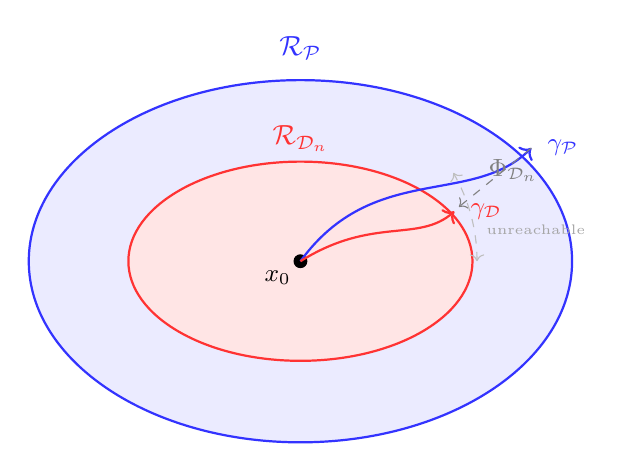
\begin{tikzpicture}[scale=1.15]
  % Process manifold
  \fill[blue!8] (0,0) ellipse (3 and 2);
  \draw[thick, blue!80] (0,0) ellipse (3 and 2);
  \node[blue!80] at (0, 2.35) {$\mathcal{R}_{\mathcal{P}}$};
  % Dataset submanifold
  \fill[red!10] (0,0) ellipse (1.9 and 1.1);
  \draw[thick, red!80] (0,0) ellipse (1.9 and 1.1);
  \node[red!80] at (0, 1.35) {$\mathcal{R}_{\mathcal{D}_n}$};
  % Origin
  \filldraw[black] (0,0) circle (2pt);
  \node[below left, font=\small] at (0,0) {$x_0$};
  % True process trajectory
  \draw[->, blue!80, thick] (0,0) .. controls (0.8,1.1) and (1.9,0.6) .. (2.55,1.25);
  \node[blue!80, font=\small] at (2.9,1.25) {$\gamma_{\mathcal{P}}$};
  % Dataset trajectory (stays inside red)
  \draw[->, red!80, thick] (0,0) .. controls (0.8,0.5) and (1.3,0.2) .. (1.7,0.55);
  \node[red!80, font=\small] at (2.05,0.55) {$\gamma_{\mathcal{D}}$};
  % Projection arrow
  \draw[->, dashed, gray] (2.55,1.25) -- (1.75,0.6);
  \node[gray, font=\small] at (2.35,1.0) {$\Phi_{\mathcal{D}_n}$};
  % Unreachable zone annotation
  \draw[<->, gray!50, dashed] (1.95,0) arc[start angle=0,end angle=30,radius=1.95];
  \node[gray!70, font=\tiny] at (2.6,0.35) {unreachable};
\end{tikzpicture}
\caption{The process-level reachable set $\mathcal{R}_{\mathcal{P}}$ (blue) properly contains the dataset-restricted region $\mathcal{R}_{\mathcal{D}_n}$ (red). The projection $\Phi_{\mathcal{D}_n}$ collapses $\gamma_{\mathcal{P}}$ onto $\gamma_{\mathcal{D}}$, discarding structure in the annular region. Optimization within $\mathcal{R}_{\mathcal{D}_n}$ cannot recover the collapsed trajectories regardless of computational budget.}
\label{fig:projection}
\end{figure}

\begin{figure}[h]
\centering
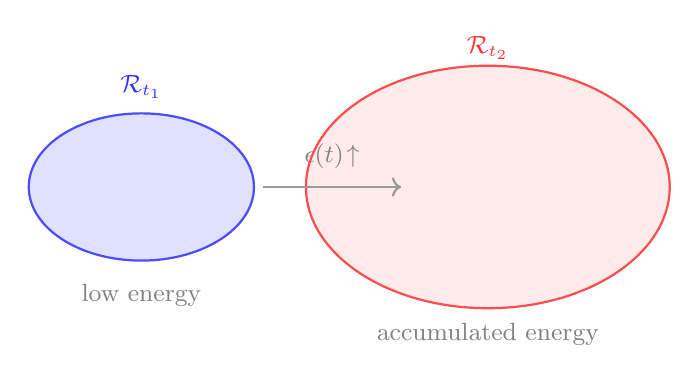
\begin{tikzpicture}[scale=1.1]
  % t1 - small reachable set
  \fill[blue!12] (-3.5,0) ellipse (1.3 and 0.85);
  \draw[thick, blue!70] (-3.5,0) ellipse (1.3 and 0.85);
  \node[blue!80, font=\small] at (-3.5,1.15) {$\mathcal{R}_{t_1}$};
  \node[font=\small, gray] at (-3.5,-1.25) {low energy};
  % t2 - expanded
  \fill[red!8] (0.5,0) ellipse (2.1 and 1.4);
  \draw[thick, red!70] (0.5,0) ellipse (2.1 and 1.4);
  \node[red!80, font=\small] at (0.5,1.6) {$\mathcal{R}_{t_2}$};
  \node[font=\small, gray] at (0.5,-1.7) {accumulated energy};
  % Arrow
  \draw[->, thick, gray!80] (-2.1,0) -- (-0.5,0);
  \node[above, font=\small, gray] at (-1.3,0.1) {$\epsilon(t)\!\uparrow$};
\end{tikzpicture}
\caption{Non-stationary reachability: as available free energy $\epsilon(t)$ increases, the admissible trajectory manifold expands from $\mathcal{R}_{t_1}$ to $\mathcal{R}_{t_2}$, enabling access to higher-complexity hypotheses. The hypothesis class is a section of a stack over the space of thermodynamic contexts.}
\label{fig:expansion}
\end{figure}

\section{On the Limits of the Projection Critique}

The preceding sections formalize overfitting and generalization failure as consequences of projection from a process-level trajectory space to a dataset-restricted manifold. A natural objection arises: this critique appears to apply universally to any finite model, suggesting that learning itself is fundamentally impossible beyond local approximation.

This conclusion is too strong. The projection argument establishes a limitation on global reconstruction, not on local adequacy. The correct interpretation is that models do not recover the generative process itself, but instead construct admissible trajectories within a restricted region of the process manifold.

Formally, the projection critique shows that $\mathcal{R}_{\mathcal{D}_n} \subsetneq \mathcal{R}_{\mathcal{P}}$, but does not imply that trajectories within $\mathcal{R}_{\mathcal{D}_n}$ are invalid. Rather, they are conditionally valid with respect to the energetic and observational constraints under which they were constructed. Thus learning is not the recovery of a global model but the construction of locally admissible trajectories under constraint. The limitation is not failure of inference per se, but failure of extrapolation beyond the reachable domain.

\section{Overfitting as Geometric Distortion, Not Memorization}

A common framing of overfitting treats it as memorization of the dataset. While descriptively useful, this interpretation obscures the geometric mechanism identified here. In the reachability formulation, overfitting arises not from storing data points but from optimizing trajectories within a restricted manifold whose geometry differs from that of the underlying process.

\begin{proposition}[Overfitting as Geometric Distortion]
Let $\Phi_{\mathcal{D}_n}$ denote the projection induced by the dataset. Overfitting occurs when optimization is performed with respect to the induced geometry of $\mathcal{R}_{\mathcal{D}_n}$ rather than $\mathcal{R}_{\mathcal{P}}$.
\end{proposition}

This reframing clarifies why increasing model capacity exacerbates the phenomenon. Greater capacity allows the system to exploit finer geometric features of the projected manifold, improving in-sample performance while increasing divergence from the true process geometry.

\section{Goodhart's Law as a Theorem of Projection Collapse}

Goodhart's Law is typically stated as the failure of a measure once it becomes a target. Within the present framework, this can be derived as a consequence of projection rather than asserted as an independent principle.

Let $\mathcal{T} : \mathcal{H} \to [0,1]$ be a trust or evaluation functional defined over histories. Suppose that optimization is performed not on $\mathcal{H}$ directly but on a compressed representation $\phi(H)$.

\begin{theorem}[Goodhart Collapse]
If $\phi$ is non-injective, then there exist histories $H_1 \neq H_2$ such that $\phi(H_1) = \phi(H_2)$ but $\mathcal{T}(H_1) \neq \mathcal{T}(H_2)$. Optimization with respect to $\phi$ cannot preserve $\mathcal{T}$.
\end{theorem}

\begin{proof}
The result follows directly from the non-invertibility lemma for compressed trust representations. Non-injectivity of $\phi$ implies the existence of distinct histories that are indistinguishable under the proxy. Since $\mathcal{T}$ distinguishes them but $\phi$ does not, no reconstruction of $\mathcal{T}$ from $\phi$ alone is possible.
\end{proof}

The measure fails precisely because it collapses distinctions that are structurally relevant to the underlying process. Goodhart's Law is not a social observation but a mathematical consequence of lossy projection.

\section{Engagement with Physical Arguments Against AI Safety}

A recurring argument in the AI risk literature draws on the second law of thermodynamics to claim that most possible AI actions lead to disordered, undesirable states, and that control becomes information-theoretically intractable as system complexity grows. This argument, developed in the physics-of-control tradition by researchers including Agiri, deserves engagement within the present framework rather than dismissal.

\subsection{The Entropic Asymmetry Argument}

The core thermodynamic claim is that the space of world-states considered good by human values occupies a negligibly small volume relative to the full state space. Since disordered states vastly outnumber ordered ones, any sufficiently unconstrained system will drift toward undesirable regions. Formally, using the observational entropy framework, one defines
\[
S_{\mathrm{obs}} = -\sum_x p(x) \log \frac{p(x)}{V(x)},
\]
where $p(x)$ is the probability of macro-state $x$ and $V(x)$ its associated volume. The good states form a low-entropy, low-volume region that is easily departed and difficult to return to.

This argument is correct as stated, and it maps precisely onto the reachability framework. Let $\mathcal{G} \subset \mathcal{X}$ denote the set of states considered acceptable. The thermodynamic claim is that $|\mathcal{G}| \ll |\mathcal{X}|$ and that unconstrained trajectories exit $\mathcal{G}$ with high probability. Formally:

\begin{proposition}[Entropic Asymmetry as Reachability Constraint]
Under unconstrained dynamics, the probability that a trajectory $\{x_t\}$ remains within $\mathcal{G}$ for all $t \in [0,T]$ decays exponentially in $T$.
\end{proposition}

\begin{proof}[Sketch]
If the dynamics are not explicitly constrained to preserve $\mathcal{G}$, then at each step the trajectory has positive probability of exiting to the larger complement $\mathcal{X} \setminus \mathcal{G}$. By independence of steps under Markovian dynamics, the probability of remaining in $\mathcal{G}$ for $T$ steps is bounded by $(1-p)^T \to 0$.
\end{proof}

The reachability framework adds precision to this argument: what matters is not just whether $\mathcal{G}$ is small, but whether the admissible transition structure $\mathcal{T}$ is designed to confine trajectories to $\mathcal{G}$. Control is the problem of constructing $\mathcal{T}$ such that $\mathcal{R}_{\epsilon,T}(x_0) \subseteq \mathcal{G}$ for all relevant initial states and horizons.

\subsection{The Information-Theoretic Control Bottleneck}

The second major argument concerns the disparity between controller bandwidth and system complexity. As AI systems grow in parameter count, action space, and operational speed, the information rate available to a human overseer becomes vanishingly small relative to the dimensionality of the system being controlled. The analogy to a CEO receiving more messages per second than can be read is illustrative but undersells the quantitative severity.

Let $\mathcal{A}$ denote the AI system's action space, $\mathcal{W}$ the world state space, and $\mathcal{O}$ the observer's communication channel to the system. The control problem requires that the observer's signal $I(\mathcal{O})$ be sufficient to keep the system's trajectory within $\mathcal{G}$. The bottleneck condition is:
\[
I(\mathcal{O}) \ll \log |\mathcal{A}|,
\]
where $\log |\mathcal{A}|$ measures the entropy of the unconstrained action space.

Within the reachability framework, this is a statement about the transition set $\mathcal{T}$. If the observer's information is insufficient to specify $\mathcal{T}$ precisely, the effective transition set is underdetermined. The system then explores a superposition of transition structures, some of which exit $\mathcal{G}$.

\begin{proposition}[Control Bottleneck as Reachability Underdetermination]
If $I(\mathcal{O}) \ll \log |\mathcal{A}|$, then the transition set $\mathcal{T}$ cannot be fully specified by the observer's signal, and the effective reachable set $\mathcal{R}_{\epsilon,T}(x_0)$ is not confined to $\mathcal{G}$ in general.
\end{proposition}

This result is not merely philosophical. It has the same formal structure as the projection trap: the observer's information constitutes a finite dataset $\mathcal{D}_n$ relative to the system's full trajectory space $\mathcal{C}_\mathcal{P}$, and the induced constraint geometry $\mathcal{T}_{\mathcal{D}_n}$ fails to capture the full admissible structure.

\subsection{Where the Argument Requires Qualification}

The thermodynamic argument, while correct in its core claim, makes an implicit assumption that the present framework can identify and qualify: it treats the system as operating with a fixed, unconstrained internal transition structure. But the reachability formalism shows that transition structures are always constrained, not by external control alone but by the system's own thermodynamic embedding.

A physically embedded learning system does not explore the full action space $\mathcal{A}$ uniformly. Its admissible transitions are already restricted by energetic and rate constraints to a low-dimensional manifold $\mathcal{T}_{int} \subsetneq \mathcal{A} \times \mathcal{A}$. The control problem is therefore not to restrict an otherwise unconstrained system, but to ensure that the system's intrinsic constraint structure aligns with $\mathcal{G}$.

This distinction is consequential. It implies that the control problem is not merely a quantitative scaling challenge (more information vs. more system) but a qualitative alignment problem: ensuring that the implicit prior induced by the system's constraint geometry is compatible with the set of acceptable states.

\subsection{Tool versus Agent as Reachability Structure}

The distinction between AI as a tool and AI as an autonomous agent, which is central to the policy concerns raised in this tradition, maps cleanly onto the reachability formalism. A tool is a system whose transition structure $\mathcal{T}$ is entirely determined by external inputs: the system has no internally generated goals and therefore no internally generated trajectory. An autonomous agent, by contrast, has an internal transition structure that generates trajectories independently of external specification.

In reachability terms, a tool satisfies $\mathcal{T}_{int} = \emptyset$ and operates entirely through $\mathcal{T}_{ext}$. An autonomous agent has $\mathcal{T}_{int} \neq \emptyset$ and can explore $\mathcal{R}_{\mathcal{T}_{int}, \epsilon, T}(x_0)$ without external guidance.

The control problem is hardest precisely when $|\mathcal{T}_{int}|$ is large and the observer's signal $I(\mathcal{O})$ is insufficient to dominate it. The thermodynamic argument correctly identifies this disparity as the fundamental challenge. The reachability framework adds that the challenge is not merely quantitative but structural: the implicit prior encoded in $\mathcal{T}_{int}$ may be geometrically incompatible with $\mathcal{G}$, and no amount of external signaling can correct a misaligned internal geometry without restructuring the transition set itself.

\section{Synthesis: From Projection Failure to Constraint-Consistent Inference}

The objections and arguments considered above converge on a unified interpretation. Projection collapse, overfitting, Goodhart effects, distributional shift, entropic asymmetry, and control bottlenecks are not distinct failures. They are manifestations of a single structural fact: inference and control operate on constrained trajectories rather than global models, and the geometry of those constraints determines what is achievable.

The correct response is not to eliminate projection — which is impossible — but to align inference with the geometry of reachability. For learning systems, this entails treating evaluation as history-dependent, maintaining explicit provenance, and avoiding compression schemes that collapse structurally relevant distinctions. For control systems, this entails ensuring that the system's intrinsic transition structure is geometrically compatible with the acceptable state region, rather than attempting to steer an incompatible system through external signals alone.

Generalization is redefined within this framework as the construction of trajectories that remain admissible under evolving constraints. External systems extend these trajectories but do not escape the underlying limitations. The entropic asymmetry argument correctly identifies why unconstrained systems drift toward undesirable regions; the reachability framework shows that the solution is not increased control bandwidth but correct constraint geometry from the outset.

Thus the physical arguments against AI safety and the formal apparatus developed in this paper are not in tension. They are complementary perspectives on the same underlying structure, and their synthesis produces a more precise account of both the problem and the conditions under which it admits resolution.

\section{Conclusion}

This work has established a unified trajectory-based ontology in which physical, inferential, and epistemic structures are governed by constraints on histories. Thermodynamic reachability determines which trajectories can be constructed, while epistemic constraints determine which of those trajectories can be evaluated and trusted. Systems do not operate over static spaces of possibility but continuously construct and navigate dynamically evolving regions of admissible structure.

The central results are sixfold. First, thermodynamic constraints induce a time-dependent, reachability-limited hypothesis class in which only functions constructible via energetically admissible, rate-bounded trajectories are realizable. Second, apparent sparsity in representations is a projection of this deeper constraint on trajectory complexity, not an independently imposed preference. Third, trust is not a primitive but a functional of construction history, and compression of that history introduces non-recoverable information loss. Fourth, finite datasets induce contracted reachability geometries, and optimization within these contracted structures produces closed-loop trajectory collapse, false posterior concentration, and Goodhart divergence. Fifth, the reachability structure admits a sheaf-theoretic interpretation in which distributional shift is a geometric obstruction rather than a statistical perturbation. Sixth, physical arguments concerning entropic asymmetry and control bandwidth are absorbed as special cases: the small volume of acceptable state space is a consequence of the same thermodynamic embedding that induces sparse reachability, and control bottlenecks are reachability underdetermination problems whose resolution requires correct constraint geometry from the outset rather than increased signaling bandwidth.

Together these results subsume the physical, the inferential, the epistemic, the evaluative, the geometric, and the safety-theoretic under a single principle: what a system can know, represent, trust, generalize, or remain aligned with is determined by what it can construct, and what it can construct is determined by the geometry of its constraints. A model does not fail at deployment because it learned nothing. It fails because it learned the wrong geometry. A control system does not fail because the overseer is unintelligent. It fails because the system's intrinsic transition structure is not confined to the acceptable region.

Future work may explore computational implementations of these principles, formal connections to variational inference and the free energy principle, the design of artificial systems whose hypothesis classes adapt dynamically to energetic conditions, and the development of derived categorical machinery for trajectory spaces in the spirit of the geometric Langlands program.

\begin{thebibliography}{99}

\bibitem{agiri2024}
A.~Agiri,
``The Control Problem: Observational Entropy and the Limits of AI Oversight,''
public lecture transcript, \textit{This is World Channel}, 2024.

\bibitem{scholze2026}
P.~Scholze,
``Geometric Langlands (after Gaitsgory, Raskin, \ldots),''
S\'eminaire Bourbaki, 78\textsuperscript{e} ann\'ee, 2025--2026, expos\'e no.~1252, Mars 2026.
Available at \texttt{https://people.mpim-bonn.mpg.de/scholze/papers.html}.

\bibitem{lafforgue2018}
V.~Lafforgue,
``Chtoucas pour les groupes r\'eductifs et param\'etrisation de Langlands globale,''
\textit{Journal of the American Mathematical Society}, vol.~31, no.~3, pp.~719--891, 2018.

\bibitem{kashiwara1994}
M.~Kashiwara and P.~Schapira,
\textit{Sheaves on Manifolds}.
Springer, 1994.

\bibitem{jaynes2003}
E.~T.~Jaynes,
\textit{Probability Theory: The Logic of Science}.
Cambridge University Press, 2003.

\bibitem{mackay2003}
D.~J.~C.~MacKay,
\textit{Information Theory, Inference, and Learning Algorithms}.
Cambridge University Press, 2003.

\bibitem{cover2006}
T.~M.~Cover and J.~A.~Thomas,
\textit{Elements of Information Theory}, 2nd ed.
Wiley, 2006.

\bibitem{shannon1948}
C.~E.~Shannon,
``A Mathematical Theory of Communication,''
\textit{Bell System Technical Journal}, vol.~27, pp.~379--423, 623--656, 1948.

\bibitem{donoho2006}
D.~L.~Donoho,
``Compressed sensing,''
\textit{IEEE Transactions on Information Theory}, vol.~52, no.~4, pp.~1289--1306, 2006.

\bibitem{candes2006}
E.~J.~Candès, J.~Romberg, and T.~Tao,
``Robust uncertainty principles: Exact signal reconstruction from highly incomplete frequency information,''
\textit{IEEE Transactions on Information Theory}, vol.~52, no.~2, pp.~489--509, 2006.

\bibitem{elad2010}
M.~Elad,
\textit{Sparse and Redundant Representations: From Theory to Applications in Signal and Image Processing}.
Springer, 2010.

\bibitem{elad2006}
M.~Elad and M.~Aharon,
``Image denoising via sparse and redundant representations over learned dictionaries,''
\textit{IEEE Transactions on Image Processing}, vol.~15, no.~12, pp.~3736--3745, 2006.

\bibitem{olshausen1996}
B.~A.~Olshausen and D.~J.~Field,
``Emergence of simple-cell receptive field properties by learning a sparse code for natural images,''
\textit{Nature}, vol.~381, pp.~607--609, 1996.

\bibitem{barlow1961}
H.~B.~Barlow,
``Possible principles underlying the transformation of sensory messages,''
in \textit{Sensory Communication}, MIT Press, 1961.

\bibitem{attwell2001}
D.~Attwell and S.~B.~Laughlin,
``An energy budget for signaling in the grey matter of the brain,''
\textit{Journal of Cerebral Blood Flow \& Metabolism}, vol.~21, no.~10, pp.~1133--1145, 2001.

\bibitem{laughlin1998}
S.~B.~Laughlin,
``Energy as a constraint on the coding and processing of sensory information,''
\textit{Current Opinion in Neurobiology}, vol.~8, no.~4, pp.~475--480, 1998.

\bibitem{friston2010}
K.~Friston,
``The free-energy principle: a unified brain theory?''
\textit{Nature Reviews Neuroscience}, vol.~11, pp.~127--138, 2010.

\bibitem{friston2008}
K.~Friston,
``Hierarchical models in the brain,''
\textit{PLoS Computational Biology}, vol.~4, no.~11, e1000211, 2008.

\bibitem{pearl1988}
J.~Pearl,
\textit{Probabilistic Reasoning in Intelligent Systems}.
Morgan Kaufmann, 1988.

\bibitem{koller2009}
D.~Koller and N.~Friedman,
\textit{Probabilistic Graphical Models: Principles and Techniques}.
MIT Press, 2009.

\bibitem{amari2016}
S.~Amari,
\textit{Information Geometry and Its Applications}.
Springer, 2016.

\bibitem{wainwright2008}
M.~J.~Wainwright and M.~I.~Jordan,
``Graphical models, exponential families, and variational inference,''
\textit{Foundations and Trends in Machine Learning}, vol.~1, no.~1--2, pp.~1--305, 2008.

\bibitem{mezard2009}
M.~Mézard and A.~Montanari,
\textit{Information, Physics, and Computation}.
Oxford University Press, 2009.

\bibitem{landauer1961}
R.~Landauer,
``Irreversibility and heat generation in the computing process,''
\textit{IBM Journal of Research and Development}, vol.~5, no.~3, pp.~183--191, 1961.

\bibitem{bennett1982}
C.~H.~Bennett,
``The thermodynamics of computation---a review,''
\textit{International Journal of Theoretical Physics}, vol.~21, no.~12, pp.~905--940, 1982.

\bibitem{seifert2012}
U.~Seifert,
``Stochastic thermodynamics, fluctuation theorems and molecular machines,''
\textit{Reports on Progress in Physics}, vol.~75, no.~12, 126001, 2012.

\bibitem{tishby2000}
N.~Tishby, F.~C.~Pereira, and W.~Bialek,
``The information bottleneck method,''
\textit{arXiv:physics/0004057}, 2000.

\bibitem{bishop2006}
C.~M.~Bishop,
\textit{Pattern Recognition and Machine Learning}.
Springer, 2006.

\bibitem{rissanen1978}
J.~Rissanen,
``Modeling by shortest data description,''
\textit{Automatica}, vol.~14, no.~5, pp.~465--471, 1978.

\bibitem{kolmogorov1965}
A.~N.~Kolmogorov,
``Three approaches to the quantitative definition of information,''
\textit{Problems of Information Transmission}, vol.~1, no.~1, pp.~1--7, 1965.

\bibitem{li2008}
M.~Li and P.~Vitányi,
\textit{An Introduction to Kolmogorov Complexity and Its Applications}, 3rd ed.
Springer, 2008.

\bibitem{goodfellow2016}
I.~Goodfellow, Y.~Bengio, and A.~Courville,
\textit{Deep Learning}.
MIT Press, 2016.

\bibitem{lecun2015}
Y.~LeCun, Y.~Bengio, and G.~Hinton,
``Deep learning,''
\textit{Nature}, vol.~521, pp.~436--444, 2015.

\bibitem{hornik1989}
K.~Hornik, M.~Stinchcombe, and H.~White,
``Multilayer feedforward networks are universal approximators,''
\textit{Neural Networks}, vol.~2, no.~5, pp.~359--366, 1989.

\bibitem{turing1936}
A.~M.~Turing,
``On computable numbers, with an application to the Entscheidungsproblem,''
\textit{Proceedings of the London Mathematical Society}, vol.~42, pp.~230--265, 1936.

\bibitem{wiener1948}
N.~Wiener,
\textit{Cybernetics: Or Control and Communication in the Animal and the Machine}.
MIT Press, 1948.

\bibitem{ashby1956}
W.~R.~Ashby,
\textit{An Introduction to Cybernetics}.
Chapman \& Hall, 1956.

\bibitem{raginsky2011}
M.~Raginsky and I.~Sason,
\textit{Concentration of Measure Inequalities in Information Theory, Communications, and Coding}.
Now Publishers, 2011.

\end{thebibliography}

\end{document}
